%\documentclass[conference]{IEEEtran}
\documentclass[conference]{IEEEtran}
\IEEEoverridecommandlockouts
% The preceding line is only needed to identify funding in the first footnote. If that is unneeded, please comment it out.
%\usepackage{cite}
%\usepackage[numbers,sort&compress]{natbib}

\usepackage{csquotes}
\usepackage[backend=biber,
            style=ieee,
            %style=numeric,
            natbib=true]{biblatex}
\addbibresource{references.bib}

\usepackage{amsmath,amssymb,amsfonts}
\usepackage{algorithmic}
\usepackage{graphicx}
\usepackage{hyperref}
\usepackage{booktabs}
\usepackage{multirow,multicol}
\usepackage{textcomp}
\usepackage{xcolor}
\usepackage{enumitem}
\usepackage{listings}
\usepackage{caption}
\usepackage{xspace}

\usepackage{booktabs}
\usepackage{multirow}
\usepackage[table]{xcolor}

% \usepackage{cite}
\usepackage{tagging}

% \usepackage{sc26repro}

\def\BibTeX{{\rm B\kern-.05em{\sc i\kern-.025em b}\kern-.08em
    T\kern-.1667em\lower.7ex\hbox{E}\kern-.125emX}}
\begin{document}

\newcommand{\textitbf}[1]{\textbf{\textit{#1}}}

% \title{LLMs as Static GPU Roofline Performance Profilers\\
% \title{Static GPU Program Cost Estimation using LLMs\\
% \title{LLMs are Static GPU Program Cost Estimators\\
% \title{LLMs are Static Roofline Triage Tools for GPU Kernels\\
\title{Off-the-Shelf LLMs are Static Roofline Triage Tools for GPU Kernels\\


% \thanks{Identify applicable funding agency here. If none, delete this.}
}

 \author{
 \IEEEauthorblockN{anonymous author(s)}
 %\IEEEauthorblockA{\textit{Virginia Tech}\\
 %Blacksburg, VA, USA\\
 %gbolet@vt.edu
 }
 
% \author{
% \IEEEauthorblockN{Gregory Bolet}
% \IEEEauthorblockA{\textit{Virginia Tech}\\
% Blacksburg, VA, USA\\
% gbolet@vt.edu}
% \and
% \IEEEauthorblockN{Giorgis Georgakoudis}
% \IEEEauthorblockA{\textit{Lawrence Livermore Natl Lab}\\
% Livermore, CA, USA\\
% georgakoudis1@llnl.gov}
% \and
% \IEEEauthorblockN{Harshitha Menon}
% \IEEEauthorblockA{\textit{Lawrence Livermore Natl Lab}\\
% Livermore, CA, USA\\
% harshitha@llnl.gov}
% \and
% \IEEEauthorblockN{Konstantinos Parasyris}
% \IEEEauthorblockA{\textit{Lawrence Livermore Natl Lab}\\
% Livermore, CA, USA\\
% parasyris1@llnl.gov}
% \and
% \IEEEauthorblockN{Niranjan Hasabnis}
% \IEEEauthorblockA{\textit{Code Metal}\\
% Boston, MA, USA\\
% niranjan@codemetal.ai}
% \and
% \IEEEauthorblockN{Kirk W. Cameron}
% \IEEEauthorblockA{\textit{Virginia Tech}\\
% Blacksburg, VA, USA\\
% cameron@vt.edu}
% \and
% \IEEEauthorblockN{Gal Oren}
% \IEEEauthorblockA{\textit{Stanford University}\\
% Stanford, CA, USA\\
% galoren@stanford.edu}
% }


\maketitle

\newcommand{\gptoss}{\texttt{GPT-OSS}\xspace}
\newcommand{\opus}{\texttt{Opus-4.6}\xspace}
\newcommand{\gptfivefour}{\texttt{GPT-5.4}\xspace}
\newcommand{\sourceonly}{\textit{source-only}\xspace}
\newcommand{\sourceSASS}{\textit{source+SASS}\xspace}
\newcommand{\pmten}[0]{$\pm10\%$\xspace}
\newcommand{\pmfifty}[0]{$\pm50\%$\xspace}
\newcommand{\bandbound}[0]{BB\xspace}
\newcommand{\compbound}[0]{CB\xspace}

% we are given a max of 150 words
% 1/3 = 50 for problem descrip 
% 1/3 = 50 for our approach
% 1/3 = 50 for final results 

\begin{abstract}
GPU kernel optimization relies on profiler feedback, but hardware access is not always available early in development.
We ask whether off-the-shelf large language models, used without task-specific training, can provide early Roofline guidance by estimating arithmetic intensity from code and build artifacts.

For each kernel's first invocation, we prompt the models to predict floating-point work and DRAM traffic, then derive arithmetic intensity.
We evaluate 254 CUDA and OpenMP kernels across four NVIDIA GPUs, comparing prompts built from pre-compilation information alone against prompts that also include post-compilation assembly.

Our results show that stronger models can provide arithmetic-intensity estimates for early triage, that post-compilation information is most helpful for half-precision estimates and for determining whether a kernel is compute-bound or bandwidth-bound, and that a cheaper model remains competitive when only source-level information is available.
To support follow-on work in this area, we also release a benchmark for this task (https://flopbench.github.io/).
% Static program cost estimation allows developers to optimize their codes without the need for hardware access, mitigating costly/infeasible profiling steps while enabling early development of performant code.
% We investigate whether large language models (LLMs) can act as accurate static cost estimators for GPU programs by estimating their Roofline Arithmetic Intensity (RAI). 
% 
% For a given GPU kernel, we ask LLMs to predict the runtime FLOP counts and DRAM bytes read/written, from which RAI follows.
% Evaluating on 254 CUDA/OpenMP GPU kernels across four NVIDIA GPUs, we comparatively study the effects of prompting with pre- and post-compilation information, such as source code and SASS instructions, respectively.
% 
% We reveal that LLMs can produce accurate RAI estimates, with the most expensive LLMs consistently producing the best estimates.
% We tease out the limitations of LLM-based static program cost estimation, alongside publishing a dataset for LLM benchmarking on this task.

%We tease out when post-compilation information is helpful, as well as the limitations of LLM-based static program cost estimation.

% For a GPU kernel’s first invocation, we ask LLMs to predict the runtime FLOP counts and DRAM bytes read/written, from which AI follows.
% We study the effect of prompting with compiler optimization information by only providing pre-compilation source code versus post-compilation SASS instructions. 
% We evaluated 1349 CUDA/OpenMP GPU kernels across four NVIDIA GPUs.
%Our results reveal that for half of the sampled kernels, LLM predictions closely match profiled metrics across architectures with only pre-compilation information.
%GPU kernel optimization is typically driven by profiler feedback, but profiling requires compiling and executing on the target hardware -- often infeasible in early development, CI, restricted clusters, or when the accelerator is unavailable.
%We investigate whether large language models (LLMs) can predict Roofline-relevant metrics directly from GPU code and run configuration, enabling fast performance triage without execution.

%We study two inference modes: (1) a structured prompt that only consumes pre-compilation artifacts (i.e.: source code), and (2) the same prompt but with post-compilation information (i.e.: assembly instructions).

%Given the rise of long-input-context LLMs, we study two inference modes: (i) a zero-shot structured prompt that consumes only pre-compilation artifacts, and (ii) the same prompt but with post-compilation SASS kernel instructions.


%Our results show that LLMs provide reasonably accurate arithmetic-intensity estimates across GPU architectures, where prompting with SASS is often preferable due to the increased prediction accuracy. 
%Additionally, we stratify the sampled kernels into various classes based on source code features.
%We find that prediction errors concentrate in kernels where compilation introduces ``hidden'' instructions and traffic not apparent in source (e.g., lowered divisions, transcendental math, vectorization).
%We quantify which code patterns drive failures and identify when adding low-level compiler artifacts (e.g., SASS) is the most beneficial.
%These findings position LLM-based “static profiling” as a low-cost, hardware-free pre-filter that complements conventional profilers by accelerating kernel triage and guiding where to spend scarce profiling and tuning time.
\end{abstract}



\begin{IEEEkeywords}
roofline, arithmetic intensity, large language models, performance, prediction, graphics processing units
\end{IEEEkeywords}



%\section{Introduction}
%\label{sec:introduction}
%
%With the growing adoption of agentic software development environments (e.g., VSCode with GitHub Copilot) and artificial intelligence coding \textit{teammates} \cite{liRiseAITeammates2025}, high-performance computing (HPC) developers are increasingly using large language models (LLMs) to help optimize code. 
%This trend has motivated a growing body of work \cite{liRecentAdvancesDeep, gongLanguageModelsCode2025} on LLM-based code optimization, where LLMs propose source-code and compiler-flag changes to improve performance on a target hardware platform.
%
%\begin{figure}[ht!]
%    \centering
%    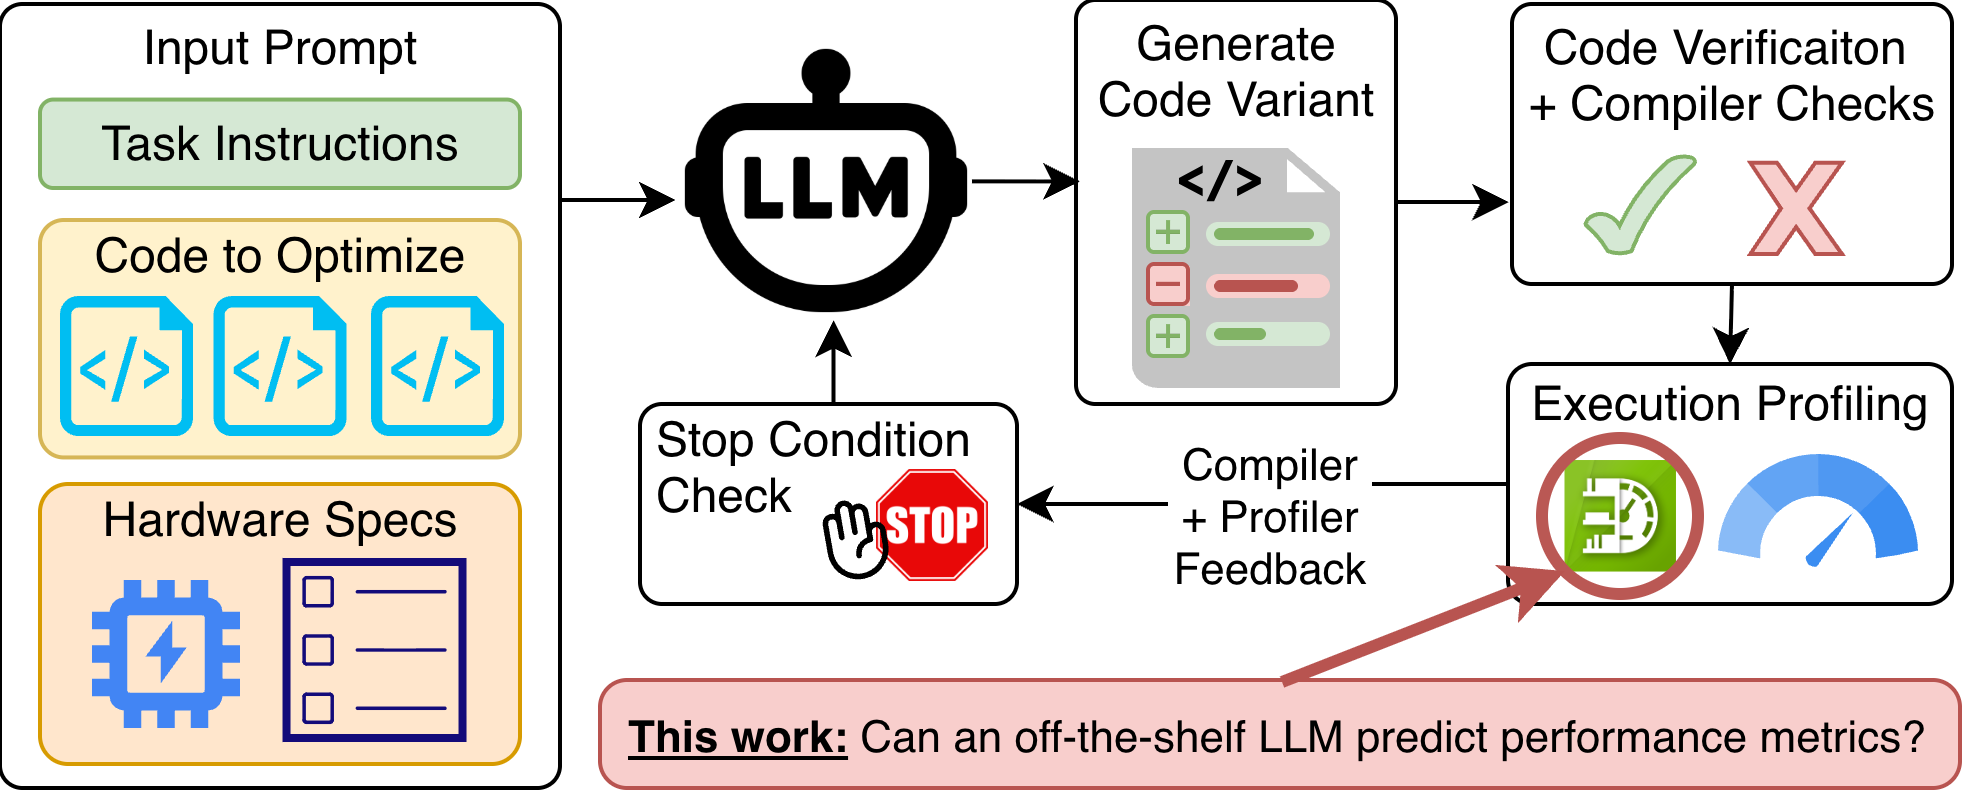
\includegraphics[width=0.95\linewidth]{figures/iterativeCodeOptimizationSimple.drawio.png}
%    \caption{Generalization of typical LLM-based iterative GPU code optimization pipelines where execution feedback from the profiler is used to inform the next code variant generation.
%    This dependence on hardware access for profiler feedback is what we address in this work.}
%    \label{fig:iterativeCodeOptimPipeline}
%\end{figure}
%
%\autoref{fig:iterativeCodeOptimPipeline} visualizes a common feedback-loop design pattern in these systems, where an LLM agent (1) proposes an optimized program variant, (2) profiles the variant on target hardware, (3) incorporates profiler feedback to propose a new variant, and (4) repeats steps 1-3 until a stopping condition is met (e.g., a performance plateau or LLM query budget). 
%Although this iterative profiler-in-the-loop approach has proven to provide better and faster code speedups, it requires repeated hardware access to execute and profile candidate programs.
%
%To reduce this dependence on hardware profiling, an alternative is to estimate performance-relevant signals that can still guide optimization decisions. 
%The Roofline performance model \cite{samuelwilliamsRooflineInsightfulVisual2009} is a standard framework for reasoning about program performance, and \textit{Arithmetic Intensity} (AI) is one of its key metrics. 
%AI captures the balance between computation and data movement, enabling optimizers to reason about whether a program is likely compute-bound or memory-bound. 
%If AI can be estimated directly from program source and artifacts, it may provide useful optimization guidance even when the target hardware is unavailable.
%
%In this paper, we investigate whether state-of-the-art (SoTA) LLMs can address this hardware-accessibility bottleneck for LLM-based GPU kernel optimization pipelines by predicting a Roofline-relevant metric---specifically, arithmetic intensity---across multiple hardware architectures, without direct hardware access. 
%We show that, in many cases, SoTA LLMs can accurately estimate the effective computation-to-communication ratio for 1700 real-world CUDA and OpenMP GPU kernels from the HeCBench suite \cite{HeCBenchMasterZjinlcf}.
%
%
%
%\textbf{Key Question.}
%This work seeks to answer the following question:
%\textit{To what extent can SoTA LLMs act as GPU Roofline performance predictors, from the perspective of predicting a kernel's arithmetic intensity?}
%
%\textbf{Research Questions.} 
%We further break down the key question into four guiding questions:
%\begin{enumerate}
%    \item \textbf{(RQ1) Generalization Across Architectures:} 
%    Can LLMs predict arithmetic intensity well across multiple architectures?
%    \item \textbf{(RQ2) Prompting Strategy:} 
%    Does agentic prompting provide better predictions than zero-shot prompting?
%    \item \textbf{(RQ3) Error Analysis:} 
%    Do certain source code features cause the LLMs to mispredict more than others?
%    \item \textbf{(RQ4) Post-Compilation Artifacts:} 
%    Does including SASS artifacts in LLM inputs improve predictions?
%\end{enumerate}
%
%
%\textbf{Contributions.}
%In summary, this paper makes the following contributions:
%\begin{itemize}
%    \item We show that LLMs can approximate profiler-derived AI for a substantial subset of kernels, enough to support early performance triage.
%    \item We demonstrate the effectiveness of prompting with SASS artifacts to improve the prediction accuracy over prompting with source code alone.
%    \item We find that a plain zero-shot prompting strategy is more cost/time efficient than using an agentic strategy to predict arithmetic intensity.
%    \item We position LLM-based static profiling as a triage tool that complements, rather than replaces, hardware profilers.
%\end{itemize}
%
%The rest of this paper is laid out as follows:
%\autoref{sec:RelatedWorks} gives some insight into the utility of the Roofline performance model for code optimization while also discussing the SoTA LLM-based optimizers that use profiler feedback in their pipelines.
%\autoref{sec:methodology} describes our approach to data collection, prompting, and evaluation metrics.
%\autoref{sec:evaluation} empirically provides answers to our four target research questions.
%Lastly, \autoref{sec:conclusion} provides a discussion of results and future directions for this work.
%
%
%%% additional citations to include in the text
%\cite{wangOmniwisePredictingGPU2025} % omniwise paper
%\cite{boletCanLargeLanguage2025} % bolet LLMs binary categorization Roofline paper
%\cite{nguyen-nhatLLMPerfGPUPerformance2024} % llmperf paper
%\cite{zhangCudaForgeAgentFramework2025} % cudaforge paper
%\cite{leeForecastingGPUPerformance2025} %neusight paper

\newcommand{\rai}[0]{RAI\xspace}

\section{Introduction}
\label{sec:introduction}

% With the growing adoption of agentic software development environments (e.g., VSCode with GitHub Copilot) and artificial intelligence coding \textit{teammates} \cite{liRiseAITeammates2025}, high-performance computing (HPC) developers are increasingly using large language models (LLMs) to help optimize code. 
% This trend has motivated a growing body of work \cite{liRecentAdvancesDeep, gongLanguageModelsCode2025} on LLM-based code optimization, where LLMs propose source-code and compiler-flag changes to improve performance on a target hardware platform.
GPU performance engineering is fundamentally profiler-driven: developers use runtime measurements and hardware counters on target accelerators to determine whether a kernel is limited by computation or data movement, often through Roofline-style analysis \cite{samuelwilliamsRooflineInsightfulVisual2009}. 
In practice, however, this workflow breaks down when the target GPU is unavailable, access is rationed on a shared system, or candidate variants cannot yet be executed end-to-end. 
At the same time, the growing adoption of agentic software development environments and AI coding \textit{teammates} \cite{liRiseAITeammates2025} has motivated a growing body of work on LLM-based code optimization \cite{gongLanguageModelsCode2025}, where LLMs propose source-code and compiler-flag changes to improve performance on a target hardware platform.


% \autoref{fig:iterativeCodeOptimPipeline} visualizes a common feedback-loop design pattern in these systems, where an LLM agent (1) proposes an optimized program variant, (2) profiles the variant on target hardware, (3) incorporates profiler feedback to propose a new variant, and (4) repeats steps 1-3 until a stopping condition is met (e.g., a performance plateau or LLM query budget). 
% Although this iterative profiler-in-the-loop approach has proven to provide better and faster code speedups, it requires repeated hardware access to execute and profile candidate programs.
\autoref{fig:iterativeCodeOptimPipeline} visualizes a common iterative feedback-loop design pattern in these systems, where an LLM agent (1) proposes an optimized program variant, (2) profiles the variant on target hardware, (3) incorporates profiler feedback to propose a new variant, and (4) repeats steps 1--3 until a stopping condition is met (e.g., a performance plateau or LLM query budget). 
Although this iterative profiler-in-the-loop approach can improve code speedups, it also tightly couples optimization quality to repeated hardware access for execution and profiling. 
This dependency is especially problematic for early-stage kernel development, where developers would ideally like useful performance guidance before investing scarce accelerator time.

% To reduce this dependence on hardware profiling, an alternative is to estimate performance-relevant signals that can still guide optimization decisions. 
% The Roofline performance model \cite{samuelwilliamsRooflineInsightfulVisual2009} is a standard framework for reasoning about program performance, and \textit{Arithmetic Intensity} (AI) is one of its key metrics. 
% AI captures the balance between computation and data movement, enabling optimizers to reason about whether a program is likely compute-bound or memory-bound. 
% If AI can be estimated directly from program source and artifacts, it may provide useful optimization guidance even when the target hardware is unavailable.
An alternative to hardware profiling is to estimate a smaller, interpretable performance signal that can still guide optimization decisions. 
%The Roofline performance model \cite{samuelwilliamsRooflineInsightfulVisual2009} is a standard framework for reasoning about program performance, and \textit{arithmetic intensity} (\textbf{AI}) is one of its central quantities. 
The Roofline performance model \cite{samuelwilliamsRooflineInsightfulVisual2009} is a standard framework for reasoning about program performance, and \textit{\textbf{R}oofline \textbf{A}rithmetic \textbf{I}ntensity} (\textbf{\rai}) is one of its central quantities. 
\rai captures the balance between computation and data movement, making it an actionable signal for deciding whether optimization efforts should focus on reducing memory traffic or improving computational efficiency. 
Recent work has begun to explore whether LLMs can reason about Roofline-relevant properties from code, including coarse categorization of kernels as memory-bound or compute-bound \cite{boletCanLargeLanguage2025}. 
Here, we push that idea further by asking whether LLMs can estimate a quantitative Roofline metric directly from program representations, even when target hardware is unavailable.

\begin{figure}[t!]
    \centering
    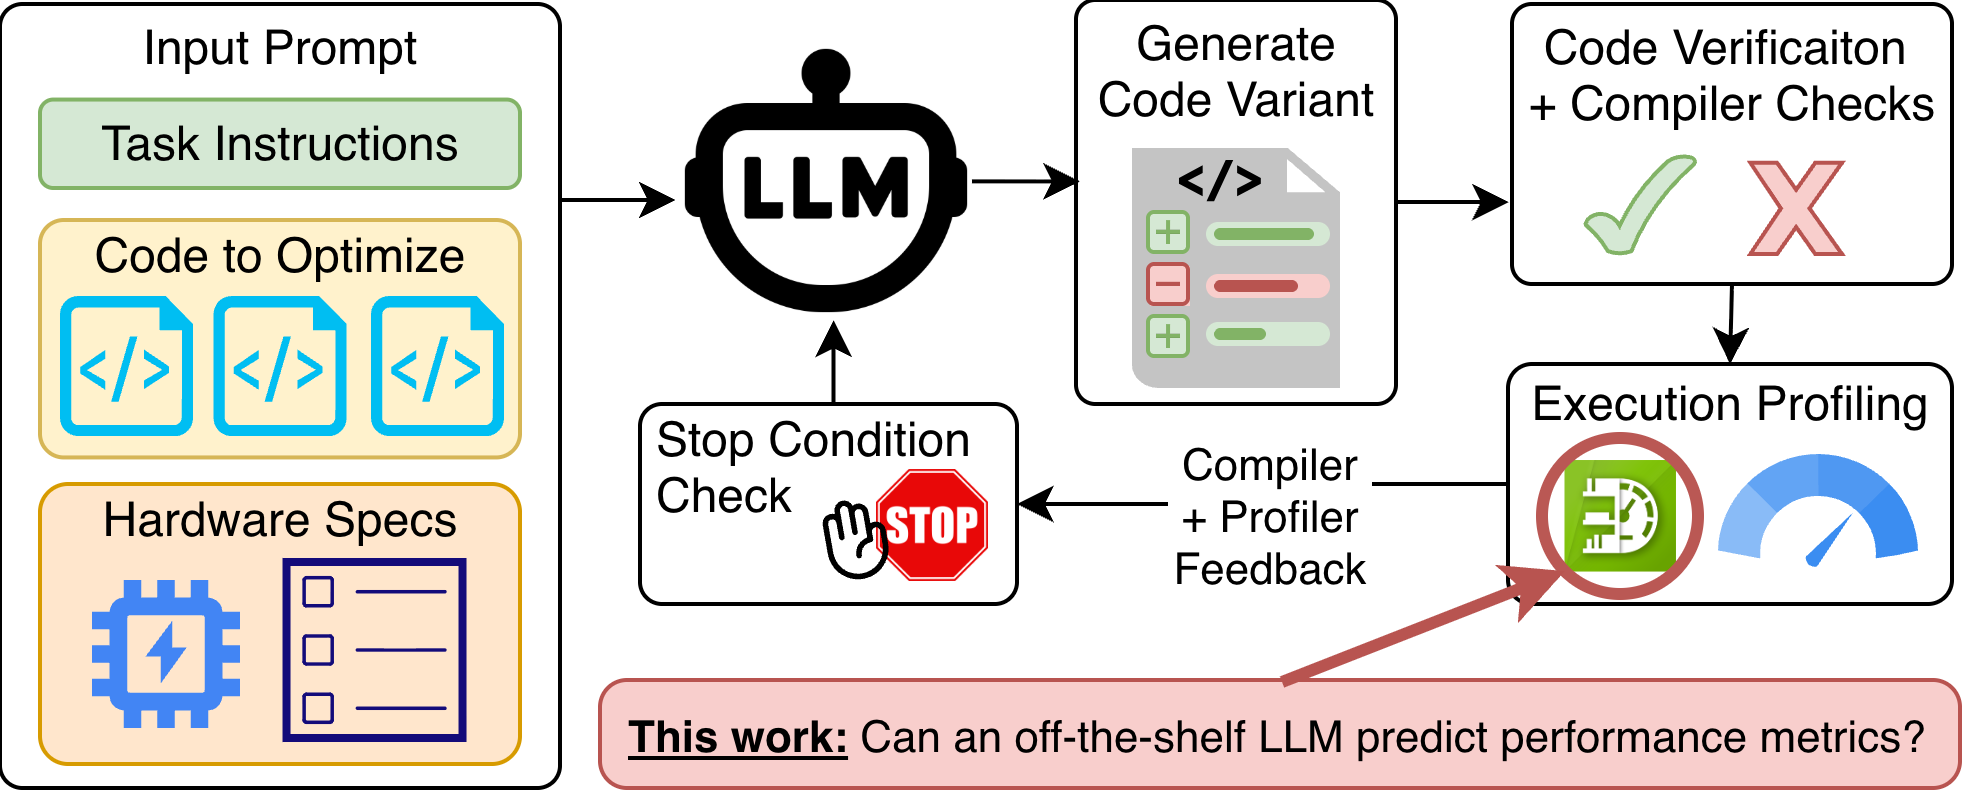
\includegraphics[width=0.95\linewidth]{figures/iterativeCodeOptimizationSimple.drawio.png}
    %\caption{Generalization of typical LLM-based iterative GPU code optimization pipelines where execution feedback from the profiler is used to inform the next code variant generation.
    %This dependence on hardware access for profiler feedback is what we address in this work.}
    \caption{Typical iterative LLM-based GPU optimization loop: generate a code variant, profile it on target hardware, and use the resulting feedback to guide the next variant.
    Our work targets the hardware-access bottleneck in this loop by estimating a Roofline-relevant signal before profiling.}
    \label{fig:iterativeCodeOptimPipeline}
\end{figure}

The main challenge with estimating \rai from source code is that effective \rai is not always obvious from source code alone: compiler passes such as lowering, instruction selection, transcendental expansion, and other low-level transformations can modify compute and memory load in ways that are not explicit from the source code \cite{alfredCompilersPrinciplesTechniques2007}. 
This makes \rai prediction a challenging test of LLMs' ability to recover profiler-relevant behavior from source-level structure alone. 
Nevertheless, we also study whether post-compilation artifacts such as SASS (i.e.: GPU assembly instructions) can help LLMs to accurately predict the \rai, as such artifacts would reveal the effects of compiler passes on the source code to the LLMs.

% In this paper, we investigate whether state-of-the-art (SoTA) LLMs can address this hardware-accessibility bottleneck for LLM-based GPU kernel optimization pipelines by predicting a Roofline-relevant metric---specifically, arithmetic intensity---across multiple hardware architectures, without direct hardware access. 
% We show that, in many cases, SoTA LLMs can accurately estimate the effective computation-to-communication ratio for 1700 real-world CUDA and OpenMP GPU kernels from the HeCBench suite \cite{HeCBenchMasterZjinlcf}.
%In this paper, we investigate whether off-the-shelf LLMs can address this hardware-accessibility bottleneck for GPU kernel optimization pipelines by predicting a Roofline-relevant metric---specifically, profiled arithmetic intensity---across multiple GPU architectures, without direct hardware access. 
%Unlike recent work that fine-tunes LLMs for GPU metric prediction~\cite{wangOmniwisePredictingGPU2025} or studies broader GPU performance modeling~\cite{leeForecastingGPUPerformance2025, nguyen-nhatLLMPerfGPUPerformance2024}, our goal is to test the zero-training regime: can LLMs, used as-is through prompting alone, reason about GPU kernel performance and serve as useful Roofline-oriented triage tools. 
In this paper, we investigate whether off-the-shelf LLMs can help address this hardware-accessibility bottleneck by predicting a single Roofline-relevant quantity---profiled arithmetic intensity---well enough to support early GPU-kernel triage without direct hardware access.
Unlike prior work that either predicts only coarse Roofline classes~\cite{boletCanLargeLanguage2025}, fine-tunes models for GPU metric prediction~\cite{wangOmniwisePredictingGPU2025}, or studies broader GPU performance modeling~\cite{leeForecastingGPUPerformance2025, nguyen-nhatLLMPerfGPUPerformance2024}, our focus is deliberately narrow: quantitative \rai prediction in the zero-training regime, using off-the-shelf LLMs through prompting alone.
Specifically, this work seeks to answer the following key question:
\textit{To what extent can off-the-shelf LLMs, used without task-specific training or fine-tuning, act as GPU Roofline triage tools by predicting a kernel's Roofline Arithmetic Intensity?}
We evaluate this question on 254 real-world CUDA and OpenMP GPU kernels from the HeCBench suite~\cite{HeCBenchMasterZjinlcf} across four different NVIDIA GPU architectures: an RTX 3080, A10, A100, and H100.
%Our results reveal that, for a substantial subset of kernels, modern LLMs can approximate effective computation-to-data-movement ratios well enough to match ground-truth profiler metrics.
We highlight three direct findings up front:
\textbf{(1)} Prompts that include post-compilation information substantially improve half-precision \rai estimates and compute/bandwidth-bound classifications for the stronger models.
\textbf{(2)} The strongest overall results come from the more capable (expensive) models, but a much cheaper model remains surprisingly competitive when only pre-compilation information is available.
\textbf{(3)} Prediction quality is not uniform: larger-cache GPUs are easier settings than smaller-cache GPUs, and prediction errors concentrate around code patterns such as division, transcendental math functions, reusable subexpressions, and loop-invariant floating-point work.

%\textbf{Key Question.}
% This work seeks to answer the following question:
% \textit{To what extent can SoTA LLMs act as GPU Roofline performance predictors, from the perspective of predicting a kernel's arithmetic intensity?}
% This work seeks to answer the following question:
% \textit{To what extent can off-the-shelf SoTA LLMs, used without task-specific training or fine-tuning, act as GPU Roofline triage tools by predicting a kernel's arithmetic intensity?}

\textbf{Research Questions.} 
We further break down the above key question into three guiding questions:
\begin{enumerate}
    \item \textbf{(RQ1) Generalization Across Architectures:} 
    Can LLMs predict Roofline Arithmetic Intensity well across multiple architectures?
    \item \textbf{(RQ2) Error Analysis:} 
    Do certain source code features cause the LLMs to mispredict more than others?
    \item \textbf{(RQ3) Post-Compilation Artifacts:} 
    Does feeding SASS artifacts to LLMs improve predictions?
\end{enumerate}


\textbf{Contributions.}
This paper makes the following contributions:
\begin{itemize}
    % \item We show that LLMs can approximate profiler-derived AI for a substantial subset of kernels, enough to support early performance triage.
    % \item We demonstrate the effectiveness of prompting with SASS artifacts to improve the prediction accuracy over prompting with source code alone.
    % \item We find that a plain zero-shot prompting strategy is more cost/time efficient than using an agentic strategy to predict arithmetic intensity.
    % \item We position LLM-based static profiling as a triage tool that complements, rather than replaces, hardware profilers.
    % \item We compare zero-shot prompting against an agentic prompting strategy and show when the additional reasoning cost of agentic interaction is, and is not, worthwhile for arithmetic-intensity prediction.

    \item We show that off-the-shelf LLMs, without task-specific training or fine-tuning, can estimate a kernel's arithmetic intensity well enough to provide useful early Roofline triage across multiple GPU architectures.
    \item We show that adding post-compilation artifacts improves prediction quality, especially for half-precision estimates and for deciding whether a kernel falls on the bandwidth- or compute-limited side of the Roofline, thereby quantifying when source-level reasoning fails to capture compiler-realized behavior.
    \item We identify where the method is (and is not) reliable by comparing inexpensive and premium LLMs across CUDA and OpenMP kernels, across GPUs with different cache regimes, and across source-code features that systematically raise prediction error.
    \item We release a benchmark for quantitative, hardware-free Roofline reasoning that includes GPU kernels, compilation and execution context, post-compilation artifacts, and profiler-derived ground truth for arithmetic-intensity prediction.\footnote{https://flopbench.github.io/}

    % \item We demonstrate that off-the-shelf LLMs can indeed estimate a kernels' arithmetic intensity across multiple GPU architectures, without any task-specific training or fine-tuning.
    % \item We show that including SASS artifacts during prompting can improve prediction accuracy over source code-only prompting, quantifying when source-level reasoning fails to capture compiler-realized behavior.
    % \item We differentiate the source code features of both CUDA and OpenMP codes that contribute to better (or worse) arithmetic intensity predictions. 
    % \item We compare and contrast the effectiveness of inexpensive and premium LLMs for the prediction task, highlighting the trade-off between query cost and prediction accuracy.
    % \item We identify a property of GPU hardware that hinders LLM prediction accuracy
    % \item We publish our dataset of GPU kernels as a benchmark that can be used to gauge LLM proficiency in this prediction task.
    
    % \item We evaluate whether off-the-shelf LLMs can estimate profiler-derived arithmetic intensity across multiple GPU architectures, without any task-specific training or fine-tuning.
    % \item We delineate the code features of both CUDA and OpenMP codes that contribute to better (or worse) prediction results.
    % \item We position LLM-based static profiling as an early performance-triage tool that complements, rather than replaces, hardware profilers.
\end{itemize}

% The rest of this paper is laid out as follows:
% \autoref{sec:RelatedWorks} gives some insight into the utility of the Roofline performance model for code optimization while also discussing the SoTA LLM-based optimizers that use profiler feedback in their pipelines.
% \autoref{sec:methodology} describes our approach to data collection, prompting, and evaluation metrics.
% \autoref{sec:evaluation} empirically provides answers to our four target research questions.
% Lastly, \autoref{sec:conclusion} provides a discussion of results and future directions for this work.
The rest of this paper is organized as follows:
\autoref{sec:RelatedWorks} reviews the utility of the Roofline performance model for code optimization, related static and learned GPU performance predictors, and recent LLM-based optimization systems that depend on profiler feedback.
\autoref{sec:methodology} describes our approach to data collection, prompting, and evaluation metrics.
\autoref{sec:evaluation} empirically answers our research questions.
Lastly, \autoref{sec:conclusion} discusses the implications of our findings and future directions for this work.




% try to also keep this to 1-1.5 pages 

%\section{Related Works} 
%\label{sec:RelatedWorks}
%
%This work falls into the realm of GPU kernel performance metric prediction using LLMs. 
%The closest neighboring realms are those of (a) using LLMs for parallel code generation/optimization, and (b) using LLMs for program analysis and execution simulation.
%We discuss existing works from our realm and its neighbors below.
%
%
%\textbf{LLMs for Parallel Code Generation.}
%
%Over the past few years, the utilization of LLMs for parallel code generation has exploded.
%The code optimization works can be largely broken up into two camps: (1) fine-tuning/training-based, and (2) out-of-the-box LLM-based.
%
%The fine-tuning works usually focus on creating a dataset of parallel codes 
%The dataset is often synthetic in nature, so extra efforts are made to 
%Given the natural language understanding of LLMs, and the complexity of \cite{talkadoshScopeAllYou2023}
%
%Talk about fine-tuned code LLMs (CodeBERT, Codex, Meta LLM Compiler, CodeGen, etc.
%
%\cite{ouyangKernelBenchCanLLMs2025}
%%In the past two years there have been multiple efforts to use LLMs for CUDA, OpenMP, OpenCL, and Triton code generation for GPUs.
%
%%\citet{ouyangKernelBenchCanLLMs2025} were one of the first that tasked LLMs to generate optimized CUDA kernels from PyTorch model architectures.
%%They demonstrated that profiler feedback significantly improves the generated codes' performance during refinement steps.
%%
%%\citet{nicholsCanLargeLanguage2024} is another work where
%%
%%\citet{wenMultiKernelBenchMultiPlatformBenchmark2025} 
%%\citet{liTritonBenchBenchmarkingLarge2025}
%%\citet{kaplanParaCodexProfilingGuidedAutonomous2026} is a more recent work, where 
%
%
%
%\textbf{RL for LLM-based GPU Code Generation.}
%
%Since the seminal DeepSeek-R1 paper \cite{} demonstrated the benefits of using reinforcement learning (RL) to fine-tune and distill LLM knowledge, a series of works sprung up using similar RL techniques to fine-tune LLMs for code-generation with an focus on execution speedup.
%
%\cite{dongKernelBlasterContinualCrossTask2026}
%\cite{nicholsIntegratingPerformanceTools2025}
%\cite{baronioKevinMultiTurnRL2025}
%%Another vein of work has been fine-tuning and creating custom LLM-based models for GPU code generation and optimization.
%
%%CUDA-L1
%%Kevin
%%Harshitha + Nichols work
%
%
%\textbf{Agentic Iterative/Feedback-Driven Code Optimization.}
%
%\cite{chenCUDALLMLLMsCan2025}
%\cite{}
%
%% High inference costs with agents
%% HPCToolKit + Hatchet paper (not sure what it was called)
%
%\textbf{LLMs for GPU Performance Prediction.}
%% Bolet
%% Omniwise
%
%
%\textbf{LLMs for Execution Simulation / Program Analysis / Trace Prediction.}
%
%\cite{lyuLargeLanguageModels2024} simulated code execution of Python, Java, C, C++ programs and 
%% Given that this work explores LLMs for performance prediction, our task is adjacent to the task of \textit{execution simulation}, where LLMs are used to predict and keep track of the internal state of a program.
%% These works are mostly Python-based, 
%% CoSm
%% REval
%% LiveCodeBench
%% PredEx
%
%
%
%
%\textbf{Shortcomings of Existing Work}
%
%\begin{enumerate}
%    \item \textbf{Limited Test Sets}
%    \item \textbf{Roofline Modeling Not Explicitly Considered}
%\end{enumerate}
%
%
%\textbf{The Roofline Performance Model.}


\section{Related Work}
\label{sec:RelatedWorks}

Our work lies at the intersection of Roofline-guided GPU performance modeling, execution-free prediction, and LLM-based code reasoning.
The closest prior work studies performance prediction without full profiler access, while adjacent areas use LLMs for HPC code generation, iterative optimization, and program-behavior reasoning.

%\textbf{Roofline modeling and static GPU performance prediction.}
%The Roofline model is a standard framework for reasoning about whether a kernel is limited by computation or data movement, and arithmetic intensity is one of its central quantities \cite{samuelwilliamsRooflineInsightfulVisual2009}. 
%Before LLMs, prior work explored predicting GPU performance without executing the target kernel, including static PTX-based execution-time estimation and learned models over PTX for performance, power, and energy prediction \cite{gargialavaniPredictingExecutionTime2018,guerreiroGPUStaticModeling2019}.
%More recent learned predictors extend this idea to unseen workloads and devices through few-shot transfer, hybrid GNN/LLM models, and deep-learning performance forecasters \cite{deyRelativePerformancePrediction2024,leeForecastingGPUPerformance2025,selvamCanLLMsEnhance2024,pannerselvamPerformancePredictionModels2025}.
%These works establish the value of execution-free prediction, but they do not ask whether off-the-shelf (not-finetuned) LLMs can estimate a quantitative Roofline quantity directly from GPU kernel source.
\textbf{Roofline modeling and static GPU performance prediction.}
The Roofline model is a standard framework for reasoning about whether a kernel is limited by computation or data movement, and arithmetic intensity is one of its central quantities \cite{samuelwilliamsRooflineInsightfulVisual2009}.
Long before LLMs, prior work studied GPU performance prediction using analytical and learned models built from program structure, microarchitectural assumptions, or low-level code features.
Early analytical models estimated execution time from memory- and thread-level parallelism or compiler-derived workflow graphs that capture effects such as divergence, coalescing, and bank conflicts \cite{hongAnalyticalModelGPU2009,baghsorkhiAdaptivePerformanceModeling2010}, while later static approaches predicted execution time directly from PTX or other compile-time features \cite{limAutotuningGPUKernels2017,alavaniPredictingExecutionTime2018,guerreiroGPUStaticModeling2019a}.
Roofline-style upper-bound analysis has also been extended to GPUs through cache-aware performance, power, and energy models \cite{lopesExploringGPUPerformance2017}, and newer predictors combine PTX features with learned models such as random forests or XGBoost, or replace execution-based profiling with static estimation of execution statistics \cite{braunSimpleModelPortable2021,emondsCUDAsapStaticallyDeterminedExecution2023,tranAccurateLatencyPredictor2025}.
Related work also explores profiling-informed analytical or machine-learning predictors, including bulk-synchronous-based models, DVFS-aware predictors, and more detailed analytical models of modern GPU cores \cite{amarisComparisonGPUExecution2016,wangGPGPUPerformanceEstimation2020,leeGCoMDetailedGPU2022}.
More recent learned predictors extend this direction to unseen workloads and devices through few-shot transfer, hybrid GNN/LLM models, and deep-learning performance forecasters \cite{deyRelativePerformancePrediction2024,leeForecastingGPUPerformance2025,selvamCanLLMsEnhance2024,pannerselvamPerformancePredictionModels2025}.
These works establish the value of execution-free prediction, but they mostly build specialized predictors for runtime, power, or energy from handcrafted models or trained feature pipelines.
Our work instead asks whether off-the-shelf LLMs can, through prompting alone, recover a quantitative Roofline signal of Arithmetic Intensity that is useful for early performance triage before profiler feedback is available.

\textbf{LLMs for HPC and parallel code understanding/generation.}
A broad line of work studies whether LLMs can better represent and generate HPC and parallel code through domain specialization, tailored tokenization, and benchmark-driven evaluation.
Early domain-specific efforts include \textit{Scope Is All You Need} and \textit{MonoCoder}, while HPC-Coder and related work show that HPC-focused corpora and fine-tuning can improve performance on parallel-code tasks \cite{talkadoshScopeAllYou2023,talkadoshMonoCoderDomainSpecificCode2023,danielnicholsModelingParallelPrograms2023,nicholsHPCCoderModelingParallel2024a}.
Other work studies compiler-oriented representations or benchmark suites for parallel and accelerator code, including Meta LLM Compiler, ParEval, KernelBench, and MultiKernelBench \cite{cumminsMetaLargeLanguage2024a,nicholsCanLargeLanguage2024,ouyangKernelBenchCanLLMs2025,wenMultiKernelBenchMultiPlatformBenchmark2025}.
Surveys and perspective papers likewise argue that HPC is a distinct setting for LLMs because correctness, hardware sensitivity, and performance portability all matter simultaneously \cite{chenLandscapeChallengesHPC2024,gongLanguageModelsCode2025}.
Relative to this literature, our goal is not to generate kernels, but to infer an interpretable performance signal from existing kernels before optimization begins.

\textbf{LLMs for iterative GPU code optimization.}
A large neighboring literature uses LLMs to improve code performance through iterative search with compilation, execution, and profiler feedback in the loop.
This includes evaluation-oriented studies such as KernelBench \cite{ouyangKernelBenchCanLLMs2025}, \texttt{robust-kbench} \cite{langeRobustAgenticCUDA2025}, and broader assessments of LLMs on HPC optimization tasks \cite{bowencuiLargeLanguageModels2025,cuiComprehensiveEvaluationLLMs2025}, as well as feedback-driven systems such as CUDA-LLM \cite{chenCUDALLMLLMsCan2025}, PerfCodeGen \cite{pengPerfCodeGenImprovingPerformance2025}, SpeedGen \cite{purschkeSpeedGenEnhancingCode2025}, WarpDrive \cite{damaniWarpDriveAgenticWorkflow}, IntelliPerf \cite{awadIntelliPerfLLMPoweredAutonomous2025}, Autocomp \cite{hongAutocompPowerfulPortable2025}, SwizzlePerf \cite{tschandSwizzlePerfHardwareAwareLLMs2025}, CudaForge \cite{zhangCudaForgeAgentFramework2025}, ParaCodex \cite{kaplanParaCodexProfilingGuidedAutonomous2026}, SysLLMatic \cite{pengSysLLMaticLargeLanguage2025}, the minimal-executable-program approach of Chu \textit{et al.} \cite{chuGPUKernelOptimization2025}, and agent-system approach in \cite{weiImprovingParallelProgram2024}.
A related training-based line uses RL or fine-tuning to optimize GPU code more effectively, including Kevin, CUDA-L1, KernelBlaster, and recent work on integrating performance tools into model reasoning \cite{baronioKevinMultiTurnRL2025,liCUDAL1ImprovingCUDA2026,dongKernelBlasterContinualCrossTask2026,nicholsIntegratingPerformanceTools2025}.
More broadly, evolutionary and autonomous search formulations such as LLM-GP and AlphaEvolve reinforce the value of iterative feedback for improving code quality and performance \cite{hembergEvolvingCodeLarge2024,novikovAlphaEvolveCodingAgent2025}.
Collectively, these works show that LLMs can optimize code when hardware feedback is available, whereas our work asks what useful guidance can be obtained before such feedback exists.
The downstream objective would be to later use LLM predictors in place of actual hardware profiling feedback to help drive these optimization tools.

\textbf{LLMs for GPU performance prediction.}
A smaller but much closer body of work uses LLMs as performance predictors rather than optimizers.
LLMPerf \cite{nguyen-nhatLLMPerfGPUPerformance2024} is an early demonstration that fine-tuned LLMs can act as GPU performance estimators for source programs.
Bolet et al. \cite{boletCanLargeLanguage2025} framed LLM-based prediction as a coarse Roofline-classification task that predicts whether kernels are compute-bound or bandwidth-bound.
More recently, Omniwise \cite{wangOmniwisePredictingGPU2025} introduced a fine-tuning pipeline for predicting several GPU kernel metrics, including bandwidth, cache behavior, GFLOPs, and arithmetic intensity, directly from code.
Our work differs by focusing on quantitative arithmetic-intensity prediction as an interpretable Roofline signal, by studying the zero-training regime with off-the-shelf models, and by explicitly analyzing the gap between source-level reasoning and compiler-realized behavior.
This distinction matters because floating-point semantics and lowered implementations of operations such as division can change effective FLOP counts in ways that are not explicit in source text \cite{IEEEStandardFloatingPoint2019,louvetNewtonRaphsonAlgorithmsFloatingpoint2010}.

\textbf{Program reasoning and code-property modeling.}
Arithmetic Intensity prediction also relates to whether LLMs can infer latent execution behavior and nontrivial code properties from source.
Prior work on code execution, predictive execution, and runtime-behavior reasoning shows that models can sometimes simulate program behavior, but often struggle as reasoning depth and trace complexity increase \cite{liuCodeExecutionPretrained2023,lyuLargeLanguageModels2024,liBlendedAnalysisPredictive2025,chenReasoningRuntimeBehavior2025}.
Benchmarks for static-analysis-style reasoning and broader code evaluation similarly show that current code LLMs remain brittle on deeper semantic tasks \cite{xieCOREBenchmarkingLLMs2025,jainLiveCodeBenchHolisticContamination2024}.
Related work further argues that text-only code LLMs often struggle to model latent code properties such as performance, motivating structured or lower-level representations when reasoning about behavior that is not directly visible in source \cite{pydaShortcomingsCodeLLMs2025}.
Our task fits naturally into this landscape because arithmetic-intensity prediction requires recovering execution-relevant behavior from source in a form that is directly useful for performance engineering.

\textbf{Gap addressed by this work.}
Taken together, prior work shows that static and learned models can predict aspects of GPU performance without execution, that LLM-based optimization systems benefit strongly from profiler feedback, and that LLMs remain imperfect at reasoning about latent program behavior.
What remains underexplored is whether off-the-shelf LLMs can serve as \emph{hardware-free Roofline triage tools} by estimating a quantitative profiler-relevant metric directly from code well enough to guide where scarce profiling and tuning effort should be spent.
Our work addresses this gap by studying Roofline Arithmetic Intensity prediction across GPU architectures, highlighting code features that make prediction harder, and identifying when post-compilation artifacts are needed to close the source-to-performance gap.



\section{Methodology}
\label{sec:methodology}


\textbf{Roofline Prediction Task.}
The Roofline's Arithmetic Intensity (\rai) is the ratio of floating-point work to DRAM traffic for a kernel invocation.
Rather than ask the models to predict \rai directly, we require them to predict the seven quantities from which \rai is derived:
\begin{itemize}
    \item grid size and block size,
    \item FP16, FP32, and FP64 operation counts, and
    \item DRAM bytes read and DRAM bytes written (on-device).
\end{itemize}
This decomposition makes the task more interpretable and helps in analyzing where a prediction fails.
For example, incorrect launch dimensions imply incorrect thread counts, which in turn propagate to FLOP and memory-traffic errors.

The launch-configuration prediction requires the model to propagate command-line inputs through the host code and recover the first executed kernel launch.
The floating-point operations count prediction then requires reasoning about thread-level work, loop trip counts, control-flow divergence, compiler optimization effects, and operations whose true cost is only partially visible at the source code level.
Finally, the DRAM-traffic prediction requires reasoning about what memory activity actually touches GPU on-board DRAM, rather than merely what appears as source-level loads and stores, including the effect of the GPU's L2 write-back cache on read and write traffic.
After the seven quantities are predicted, we compute \rai separately for FP16, FP32, and FP64 by dividing the predicted FLOP count by the predicted total DRAM bytes moved.
Given a FLOP precision $\texttt{FPXX} \in \{\texttt{FP16}, \texttt{FP32}, \texttt{FP64}\}$, we compute the \rai as follows:
\[
\texttt{\rai}_{\texttt{FPXX}} = \frac{\texttt{FLOP\_Count}_{\texttt{FPXX}}}{\texttt{Bytes\_Read} + \texttt{Bytes\_Written}}.
\]

%\subsection{Benchmark Selection}

%\textbf{Benchmark Selection.} 
%To answer our RQs, we decided to use CUDA and OpenMP codes, as they are two of the most popular GPU programming paradigms \cite{???}.
%Given the diversity of the C++ language and the GPU codes that can be written with it, we turn to the HeCBench suite \cite{HeCBenchMasterZjinlcf} to source a smorgasbord of benchmarks for our experiments.
%We built and profiled 586 HeCBench programs, of which 340 are CUDA, and 246 are OpenMP codes.
%In total, we sampled 1349 GPU kernels: 849 CUDA (built with the \texttt{nvcc} compiler), and 500 OpenMP \texttt{target offload} kernels (built with the \texttt{clang++} compiler).
%We purposely do not balance the CUDA and OpenMP codes in our dataset, to maintain a reflection of reality; these codes range from simulation to math to algorithms codes, so we feel our selection cast a wide-enough net to make conclusions that are broadly applicable to other un-tested CUDA/OpenMP codes.
\textbf{GPU Benchmark Selection.}
%To answer our research questions, we study CUDA and OpenMP GPU programs, two widely-adopted accelerator programming models \cite{kadoshQuantifyingOpenMPStatistical2023}.
%We draw our workloads from the HeCBench suite \cite{HeCBenchMasterZjinlcf, jinBenchmarkSuiteImproving2023}, which contains a broad range of simulation, mathematical, and algorithmic benchmarks.
We study CUDA and OpenMP GPU programs, two widely-adopted accelerator programming models \cite{kadoshQuantifyingOpenMPStatistical2023}, using workloads from the HeCBench suite \cite{HeCBenchMasterZjinlcf, jinBenchmarkSuiteImproving2023}.
From this suite, we build and profile 254 GPU kernels across two runtimes: 155 CUDA and 99 \texttt{target offload} OpenMP kernels.
We preserve the suite's natural CUDA/OpenMP composition rather than artificially balancing the two groups so the study reflects a realistic benchmark mix.
% We intentionally preserve the natural CUDA/OpenMP composition of the suite rather than artificially balancing the two groups, so that the study reflects a realistic mix of available GPU benchmark codes.

%These programs yield 1349 analyzed GPU kernels in the final paper dataset, consisting of 849 CUDA kernels and 500 OpenMP \texttt{target offload} kernels.


\begin{table}[ht]
\centering
\caption{Hardware Specs of Sampled GPUs.}
\label{tab:gpu_specs}
\scriptsize
\setlength{\tabcolsep}{3pt}
\renewcommand{\arraystretch}{1.05}
\resizebox{\columnwidth}{!}{%
\begin{tabular}{@{}p{0.35cm}p{3.25cm}cccc@{}}
\toprule
 &  & \textbf{RTX 3080 (PCIe)} & \textbf{A10 (PCIe)} & \textbf{A100 (SXM4)} & \textbf{H100 (SXM5)} \\
\midrule
 & Base architecture & Ampere (GA102) & Ampere (GA102) & Ampere (GA100) & Hopper (GH100) \\
 & Compute capability & 8.6 & 8.6 & 8.0 & 9.0 \\
 & Base Mem.\ Frequency (MHz) & 9500 & 6251 & 1215 & 1313 \\
 & Base Core Frequency (MHz) & 1440 & 885 & 1095 & 1590 \\
 & SM Count & 68 & 72 & 108 & 132 \\
 & Memory Type & GDDR6X & GDDR6 & HBM2e & HBM3 \\
 & TDP (W) & 320 & 150 & 400 & 700 \\
 & Global Memory Size (GB) & 10 & 24 & 40 & 80 \\
 & Memory Bandwidth (GB/s) & 760 & 600 & 1555 & 3360 \\
 & L2-cache size (MB) & 5 & 6 & 40 & 50 \\
\midrule
\multirow{3}{*}{\rotatebox[origin=c]{90}{\textbf{Per-SM}}}
 & L1-cache size (KB) & 128 & 128 & 192 & 256 \\
 & CUDA cores & 128 & 128 & 64 & 128 \\
 & Shared memory (bytes) & up to 100\,KB & up to 100\,KB & up to 164\,KB & up to 228\,KB \\
\midrule
\addlinespace
%\multirow{3}{*}{\rotatebox[origin=c]{90}{\textbf{Peak Perf.}}}
\multirow{3}{*}{\rotatebox[origin=c]{90}{\textbf{\begin{tabular}{@{}c@{}}Peak Perf.\\(TFLOP/S)\end{tabular}}}}
 & \ \ FP16: Half-Precision & 30.55 & 15.62 & 77.97 & 133.82 \\
 & \ \ FP32: Single-Precision & 30.55 & 15.62 & 19.49 & 66.91 \\
 & \ \ FP64: Double-Precision & 0.477 & 0.244 & 9.75 & 33.45 \\
 & \\
\midrule
\multirow{4}{*}{\rotatebox[origin=c]{90}{\textbf{\begin{tabular}{@{}c@{}}Balance Pt.\\(FLOP/byte)\end{tabular}}}}
 & \\
 & \ \ FP16: Half-Precision & 40.20 & 26.03 & 50.14 & 39.83 \\
 & \ \ FP32: Single-Precision & 40.20 & 26.03 & 12.53 & 19.91 \\
 & \ \ FP64: Double-Precision & 0.63 & 0.41 & 6.27 & 9.96 \\
 & \\
\bottomrule
\end{tabular}%
}
\end{table}


%\textbf{Hardware Selection.}
%We profiled the aforementioned codes on four GPUs: an NVIDIA RTX 3080, A10, A100, and H100.
%\autoref{tab:gpu_specs} provides a high-level comparison of the four GPUs.
%Note how we profile across three different compute-capabilities (\texttt{sm\_80}, \texttt{sm\_86}, \texttt{sm\_90}), with varying memory types/sizes, bandwidths, and peak performances.
%We selected these systems to maximize our work's applicability, as these GPUs were released multiple years apart, and are widely available on consumer/cloud-based platforms \cite{???}.
\textbf{Hardware Selection.}
We profile the benchmark suite on four NVIDIA GPUs: an RTX 3080, A10, A100, and H100.
As summarized in \autoref{tab:gpu_specs}, these devices span three compute capabilities, multiple memory technologies, and substantially different bandwidth and peak-throughput regimes, allowing us to test whether LLM-based arithmetic-intensity prediction generalizes across distinct deployment settings.

%\autoref{tab:gpu_specs} summarizes the hardware characteristics used in the study.
%Together, these devices span three compute capabilities (\texttt{sm\_80}, \texttt{sm\_86}, and \texttt{sm\_90}), multiple memory technologies, and substantially different bandwidth and peak-throughput regimes.
%This diversity is important because our objective is not to characterize a single GPU, but to test whether LLM-based arithmetic-intensity prediction generalizes across distinct architectural generations and deployment settings.



%\textbf{Profiling Design Decisions.}
%W.r.t profiling 1349 GPU kernels, we made some \textbf{\textit{simplifying design decisions}} to avoid exploding our exploration space:
%\begin{enumerate}[label=(\textbf{\arabic*})]
%    \item Profile with the base/default system clock frequencies
%    \item Sample only the first invocation of each kernel 
%    \item Only consider DRAM Arithmetic Intensity (AI)
%\end{enumerate}
%\textit{\textbf{Decision (1)}} was made to minimize the AI prediction space, as peak performance (TFLOP/s) of a system changes w.r.t clock speed, which can change a machine's balance point, altering the definition of when a kernel is considered bandwith/compute bound.
%By keeping the same balance points across profiled codes on a GPU, we can equally compare AI prediction and memory-boundedness classification accuracy.
%\textit{\textbf{Decision (2)}} was made in the interest of not complicating the prediction task.
%The AI of a GPU kernel is profiled for each invocation, this value can change across repeat kernel invocations due to cache-reuse and cross-kernel temporal dependencies. 
%Expecting the LLMs to account for these effects is an additional expectation that complicates the prediction task and subsequent failure mode analysis.
%We stick to asking the LLMs to predict the AI of only the first kernel invocation, as this task proves challenging enough for SoTA LLMs.
%\\\textbf{\textit{Decision (3)}} was made again to shrink the AI prediction space.
%The Roofline model can be expanded so the LLMs predict the AI at each of the caches of a system \cite{ilicCacheawareRooflineModel2014} however, this requires that the LLMs reason about cache reads/writes at each cache level to produce accurate AI predictions.
%When only considering the DRAM Roofline, the LLMs are already expected to reason about DRAM reads/writes that go through an L2 write-back cache; to expect even more reasoning about evictions at the L1 and L2 cache levels only further complicates the task.
%For simplicity of the task space, we keep the above three design decisions, leaving their further analysis as future work.
\textbf{Profiling Design Decisions.}
To keep the prediction task well-defined, we make three simplifying design decisions:
\begin{enumerate}[label=(\textbf{\arabic*})]
    \item profile each GPU at its base/default clock settings,
    \item analyze only the first invocation of each kernel within an executable run, and
    \item restrict the study to DRAM arithmetic intensity.
\end{enumerate}
%Decision (1) keeps each GPU's Roofline balance points fixed throughout the study, which makes cross-kernel and cross-architecture comparisons consistent.
Decision (1) keeps each GPU's Roofline balance points fixed, making cross-kernel and cross-architecture comparisons consistent.
Decision (2) avoids requiring the models to reason about inter-invocation cache reuse and cross-kernel temporal effects, both of which can change inter-invocation traffic.
Decision (3) limits the target to the DRAM-level Roofline rather than a cache-aware variant \cite{ilicCacheawareRooflineModel2014}, allowing us to focus on a single, actionable notion of arithmetic intensity while leaving finer-grained cache-level prediction as a further technical refinement.


\begin{table}[b!]
\centering
\caption{Sampled LLMs sorted by release date with corresponding input/output token costs (as-of March 2026)}
\label{tab:llm_comparison}
\scriptsize
\setlength{\tabcolsep}{3pt}
\renewcommand{\arraystretch}{1.05}
\resizebox{\columnwidth}{!}{%
\begin{tabular}{@{}p{2.2cm}p{1.6cm}p{2.0cm}p{1.5cm}@{}}
\toprule
\textbf{\vfill Model} & \textbf{\vfill Release Date} & \textbf{1e6 Token Cost\newline (in / out)} & \textbf{Max Tokens (in / out)} \\
\midrule
% % GPT-5.1 Codex Mini      & 2025-11-13 & \$0.25 / \$2    & 300K / 100K \\
% % GPT-5.2                 & 2025-12-10 & \$1.75 / \$14   & 272K / 128K \\
% Claude Opus 4.6         & 2026-02-04 & \$5 / \$25      & 872K / 128K \\
% % Claude Sonnet 4.6       & 2026-02-17 & \$3 / \$15      & 936K / 64K \\
% % Gemini 3.1 Pro          & 2026-02-19 & \$2 / \$12      & 983K / 66K \\
% % GPT-5.3 Codex           & 2026-02-24 & \$1.75 / \$14   & 272K / 128K \\
% Gemini 3.1 Flash Lite   & 2026-03-03 & \$0.25 / \$1.50 & 983K / 66K \\
% GPT-5.4                 & 2026-03-05 & \$2.50 / \$15   & 922K / 128K \\
% GPT-5.1 Codex Mini      & 2025-11-13 & \$0.25 / \$2    & 300K / 100K \\
% GPT-5.2                 & 2025-12-10 & \$1.75 / \$14   & 272K / 128K \\
GPT-OSS 120B             & 2025-08-05 & \$0.039 / \$0.19 & 131K / 131K \\
Claude Opus 4.6         & 2026-02-04 & \$5 / \$25      & 872K / 128K \\
% Claude Sonnet 4.6       & 2026-02-17 & \$3 / \$15      & 936K / 64K \\
% Gemini 3.1 Pro          & 2026-02-19 & \$2 / \$12      & 983K / 66K \\
% GPT-5.3 Codex           & 2026-02-24 & \$1.75 / \$14   & 272K / 128K \\
% Nemo 3 Nano 30B     & 2025-12-14 & \$0.05 / \$0.20 & 210K / 52K \\
% Gemini 3 Flash          & 2025-12-17 & \$0.50 / \$3    & 983K / 66K \\
% Gemini 3.1 Flash Lite   & 2026-03-03 & \$0.25 / \$1.50 & 983K / 66K \\
GPT-5.4                 & 2026-03-05 & \$2.50 / \$15   & 922K / 128K \\
% GPT-5.4 Nano            & 2026-03-17 & \$0.20 / \$1.25 & 272K / 128K \\
\bottomrule
\end{tabular}%
}
\end{table}

%\textbf{Dataset Creation.}
%When profiling the 1349 kernels on each GPU, we used NVIDIA's Nsight Compute \texttt{ncu} \cite{4NsightCompute} with \texttt{--set full} flag to gather all the performance counter data for each first invocation.
%We gathered 3 repeat sample invocations of each kernel's executable using the default HeCBench-provided command-line arguments.
%For each kernel, these 3 samples had all their Roofline-related counter metric values averaged to account for any noise during execution.
%
%Once we had the counter data collected, we also scraped all the executables to extract their SASS assembly sections for each kernel via \texttt{cuobjdump}.
%When extracting SASS, we made sure to include the SASS of all the functions called by a kernel (e.g: floating point division slowpaths) to offer a complete picture of the instructions that could be executed.
%
%We next extracted the compile commands used for each executable, as many use pre-processor defines that should be included in LLM prompting to guarantee correct reasoning about source code.
%Given the extracted compile commands, we also scraped the source codes of each executable using the files listed in their compilation commands, making sure to also scrape relevant header files used in compilation.
%This allowed us to include the minimum necessary set of source code files to build/reason about each sampled executable.
%
%\autoref{???} shows an overview of this data collection process.
%Overall, the 1349 kernels profiled across 4 GPUs resulted in a dataset of 5396 datapoints to query, allowing us to study how the LLMs predict the arithmetic intensity of many GPU kernels across 4 different devices.

\begin{figure}[ht]
    \centering
    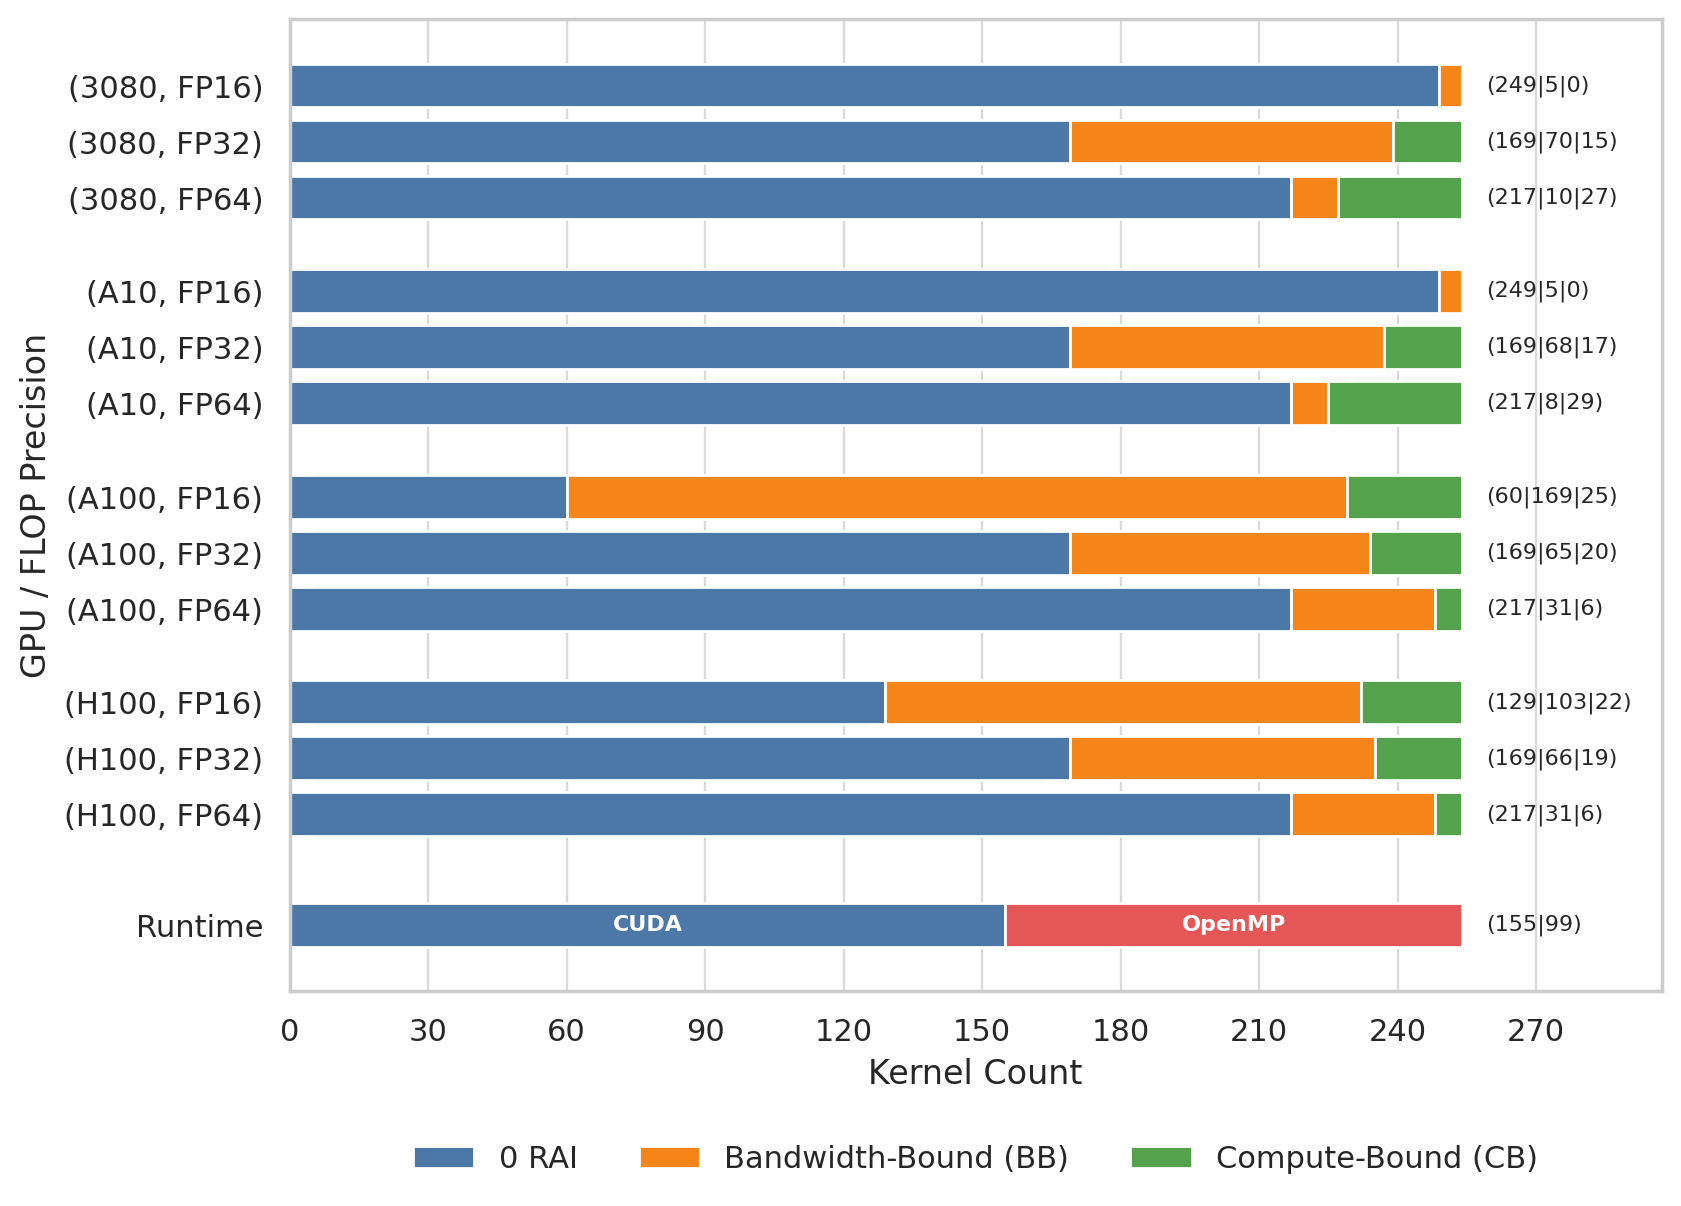
\includegraphics[width=0.95\linewidth]{figures/figure6_expected_rai_distribution_by_gpu_precision.png}
    \caption{Distribution of the profiled arithmetic-intensity classes used later in the paper, split by GPU and floating-point precision.
    Most kernels have zero \rai, while the A100 and H100 contain many more non-zero FP16 cases, motivating evaluation across multiple GPUs rather than a single device.}
    %\caption{Distribution of Bandwidth-Bound and Compute-Bound kernels profiled on each GPU at each FLOP precision.
    %There is a special case of 0 \rai, where a kernel does no FLOP work; this makes up the majority of the kernels at each FLOP precision.
    %There are a total of 254 kernels, whose \rai values vary between GPUs, causing an imbalanced dataset with more CUDA kernels than OpenMP kernels.
    %}
    \label{fig:datasetDistribution}
\end{figure}



\textbf{Dataset Creation.}
For each kernel on each GPU, we collect profiling data with NVIDIA Nsight Compute \texttt{ncu} \cite{4NsightCompute} using the \texttt{--set full} configuration.
We execute each benchmark three times with the default HeCBench command-line arguments and retain profiler statistics for the first invocation of the target kernel in each run.
We then average the Roofline-relevant counters across the three samples to reduce run-to-run noise.

From these profiling runs, we retain the quantities required for arithmetic-intensity analysis: execution time, DRAM bytes read, DRAM bytes written, and FP16/FP32/FP64 operation counts.
For the 254 profiled kernels, \autoref{fig:datasetDistribution} shows the distribution of the Bandwidth-Bound (BB) and Compute-Bound (CB) profiling results for each GPU/FLOP-precision. 
The profiled \rai values are used as ground-truth when querying LLMs to predict \rai.
We note that the majority of the kernels do not perform any FLOPs, resulting in a profiled value of 0 \rai. 
We also note that the A100 and H100 GPUs have many more non-zero FP16-\rai values due to how the compiler injects many more FP16 instructions into their kernel binaries.
These architectural discrepancies highlight the need to study LLM-based \rai predictions across multiple devices.

%We also retain only kernels with valid profiling data on all four GPUs, so that each kernel can be compared consistently across architectures.

In addition to the counter data, we also extract post-compilation artifacts needed for prompting.
We use \texttt{cuobjdump} to collect SASS sections for each target kernel, including relevant helper functions reached by the kernel body (for example, slowpaths used to implement division or transcendental operations).
We also extract the compilation commands for each executable and use them to recover the corresponding source files and relevant headers.
This produces the minimal source-and-artifact bundle needed for the model to reason about a kernel's launch configuration, floating-point work, and DRAM traffic.

\autoref{fig:datasetCreation} shows an overview of this data collection process.
After filtering to kernels with complete four-GPU coverage, the resulting dataset contains 254 kernels evaluated on four devices, yielding 1016 kernel-GPU datapoints to query for each LLM.

\begin{figure}
    \centering
    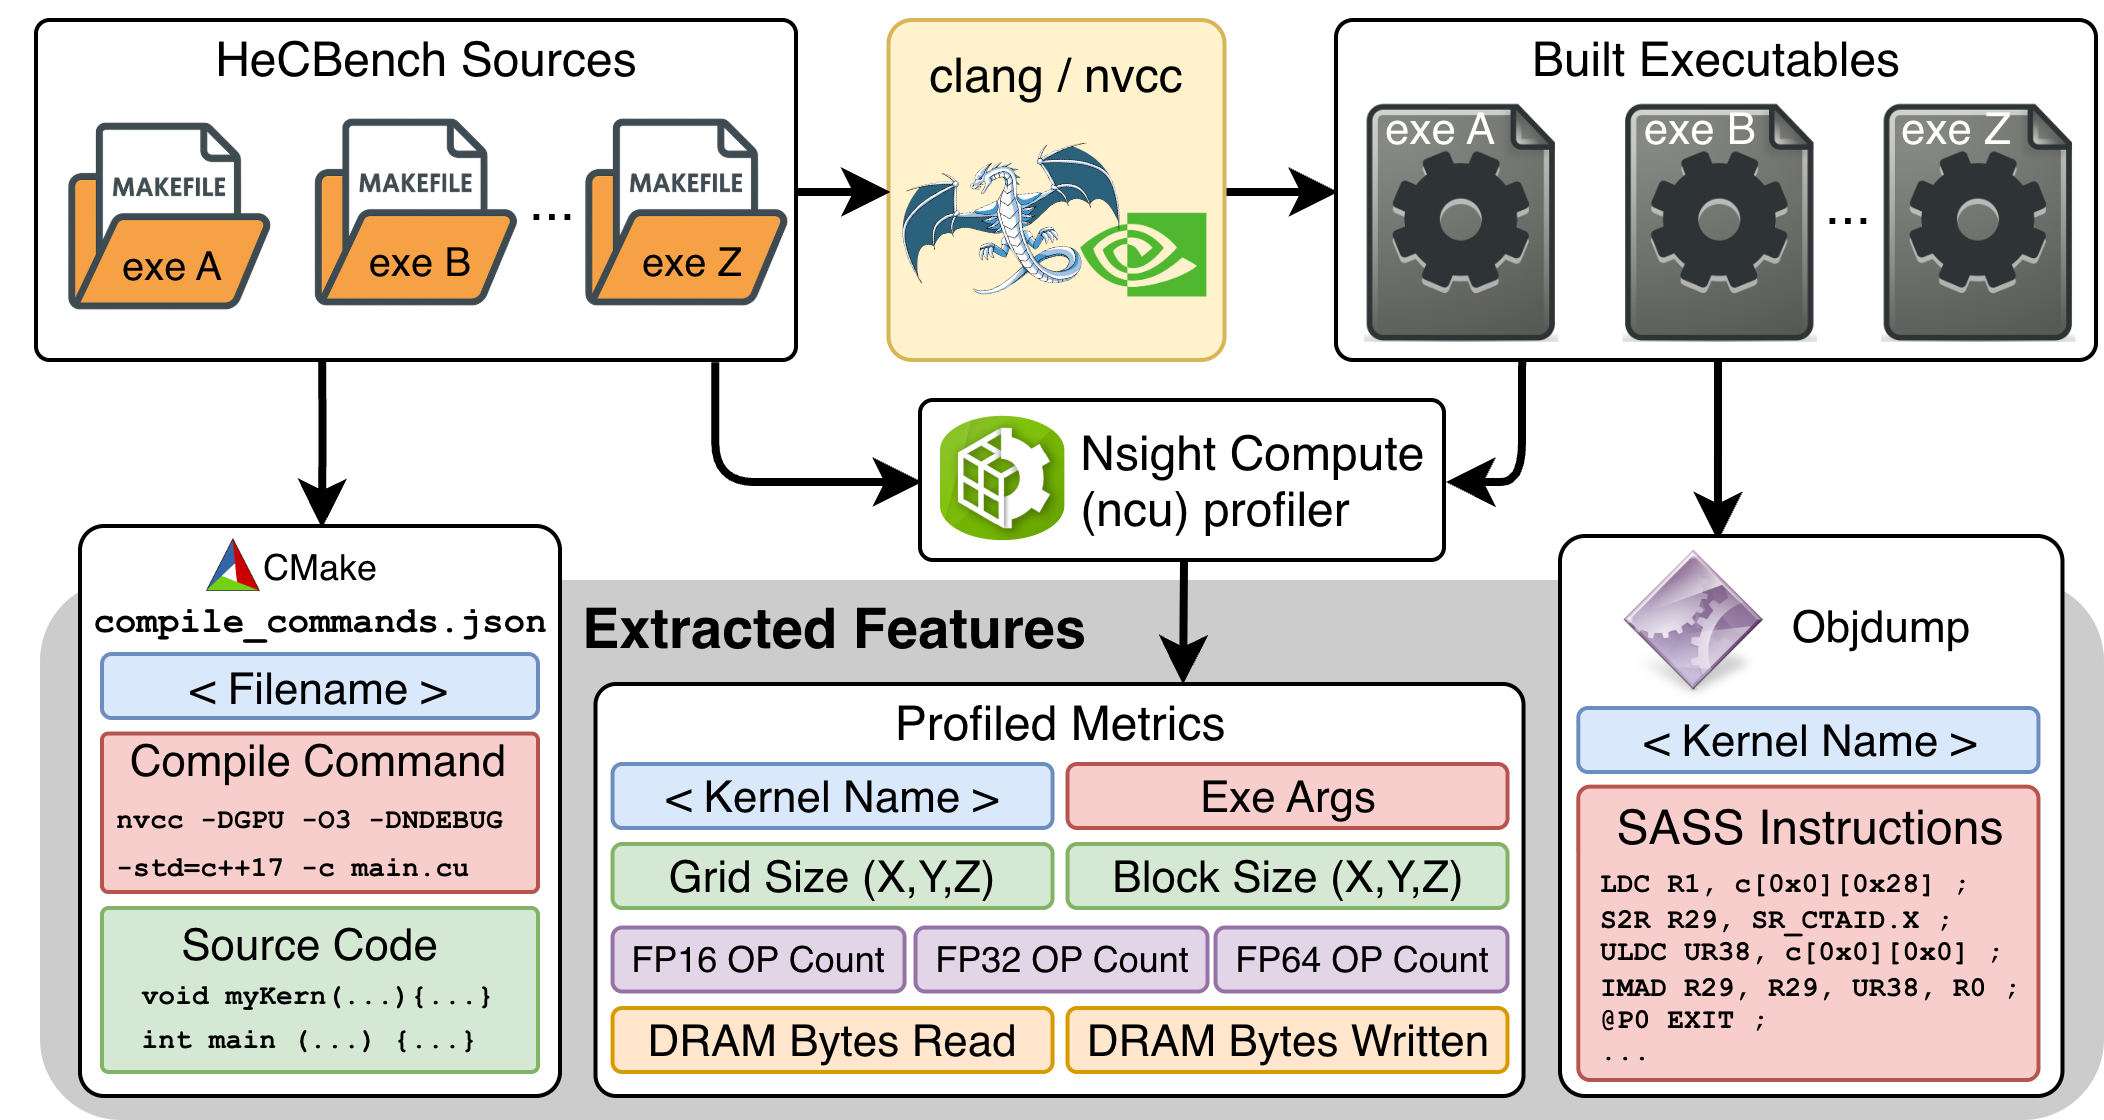
\includegraphics[width=0.95\linewidth]{figures/datasetCreation.png}
    \caption{Dataset-construction pipeline used in this work. 
    For each target kernel, we build the executable, recover the source files, compilation commands, runtime arguments, and SASS, and profile the first invocation to obtain the floating-point and DRAM-traffic ground truth used for prediction.}
    %\caption{The kernel source scraping and profiling approach used in this work.
    %We build CUDA and OpenMP executables from the HeCBench suite, extracting compilation commands, source code, execution metric, and SASS instruction features to use as inputs to the LLMs for static performance prediction.}
    \label{fig:datasetCreation}
\end{figure}


\textbf{Sampled LLMs.}
\autoref{tab:llm_comparison} lists the three models studied in this work: \opus, \gptfivefour, and the cheaper open-source baseline \gptoss.
We focus on the two frontier models to test what off-the-shelf systems can provide without task-specific training, while \gptoss serves as a cost baseline.
This baseline is roughly 100 times cheaper to query than \gptfivefour and \opus.
%\autoref{tab:llm_comparison} lists the LLMs studied in this work.
% Because we have a thousand kernel-GPU combinations, querying the leading LLM models can be quite expensive.
% We limit our comparison to two leading frontier models: Anthropic's \texttt{Opus-4.6} and OpenAI's \texttt{GPT-5.4}.
% Our goal is to evaluate what off-the-shelf models can provide without task-specific training.
% In contrast to the two expensive closed-source models, we studied OpenAI's \texttt{GPT-OSS 120B}, an open-source model released in August of 2025.
% The \gptoss model serves as cost-effective baseline of comparison, as it is 2 orders of magnitude cheaper to query than \gptfivefour and \opus.


\begin{figure}[t!]
    \centering
    
\includegraphics[width=0.9\linewidth]{figures/promptingApproach.png}
    \caption{Per-kernel prompting workflow used for arithmetic-intensity prediction.
    Each query includes the kernel identifier, source code, build context, runtime arguments, and GPU specifications; a second prompt setting additionally includes post-compilation SASS so we can measure how much compiler-realized behavior improves predictions.}
    %\caption{The direct prompting approach studied in this work. 
    %We supply pre-compilation information such as: the target kernel name for prediction, source code including the kernel definition and \texttt{main()} entrypoint of the program, executable arguments, compilation commands, and GPU hardware specification. 
    %We expect the LLM to predict the arithmetic intensity of a program by explicitly counting the number of FLOPs and DRAM Reads/Writes to calculate \rai. 
    %We perform the same queries, but with SASS instructions included to study the influence of post-compilation artifacts on predictions.}
    \label{fig:promptingApproach}
\end{figure}




\textbf{Prompting Approach.}
\autoref{fig:promptingApproach} visualizes our prompting workflow.
Each query supplies the model with the information needed to reason about one target kernel on one target GPU.
The prompt includes: (1) the target kernel name in both mangled and demangled form, (2) the compilation commands, (3) the relevant source files and headers, (4) the executable command-line arguments, (5) the target GPU hardware specifications, and (6) optional kernel-relevant SASS sections.

The kernel identifier is provided in both mangled and demangled forms because low-level artifacts such as SASS refer to mangled symbol names, while source-level reasoning is easier in demangled form.
For OpenMP kernels, we additionally preserve the source-level location information needed to disambiguate the target offload region.
This is important because a single executable may contain multiple kernel definitions, but the model is asked to reason about only one of them.

Compilation commands are included because macros, include paths, and optimization flags can materially affect both the visible source and the compiled behavior.
The associated source files are embedded directly into the prompt and wrapped in XML-style tags so the model can reason over the exact code used to build the executable.
For the source+SASS setting, we additionally provide the kernel's SASS sections, including relevant helper routines, to test whether post-compilation artifacts improve arithmetic-intensity prediction beyond source-only prompting.

The prompt is divided into a system message and a task-specific message.
The system message defines the prediction task and output constraints, while the task-specific message contains the kernel, source, build, runtime, and hardware context.
We enforce structured output through tool calling so that each response returns the seven predicted quantities together with short explanations for each one.
These explanations support both sanity checking and later error analysis.
A full prompting input and output example is available in Appendix \autoref{sec:llmPrompts}.




\textbf{Code Feature Voting.}
In order to understand what causes failures in our \rai predictions, we automatically flagged source code features that could introduce \textit{hidden} FLOPs or DRAM read/write ops post-compilation, causing the LLMs to struggle at deriving proper thread counts, FLOP counts, and memory accesses.
To do this flagging procedure, we fed each source code multiple times into the cheapest LLMs to vote for the presence or absence of these trouble-some code features.
\autoref{fig:llmVotingScheme} visualizes this voting scheme, where we query the \texttt{Nemo 3 Nano}, \texttt{Gemini 3 Flash}, \texttt{Gemini 3.1 Flash Lite}, and \texttt{GPT 5.4 Nano} three times for each source code, for a total of 12 votes to decide each feature. 
We consider a code feature as \textit{present} if more than 50\% of the votes flag it.
The code features were identified by a human expert as contributing to mispredicted \rai. 
Each code feature and it's respective description are detailed in Appendix \autoref{sec:codeFeatureCategoriesAppendix}.

\begin{figure}[t!]
    \centering
    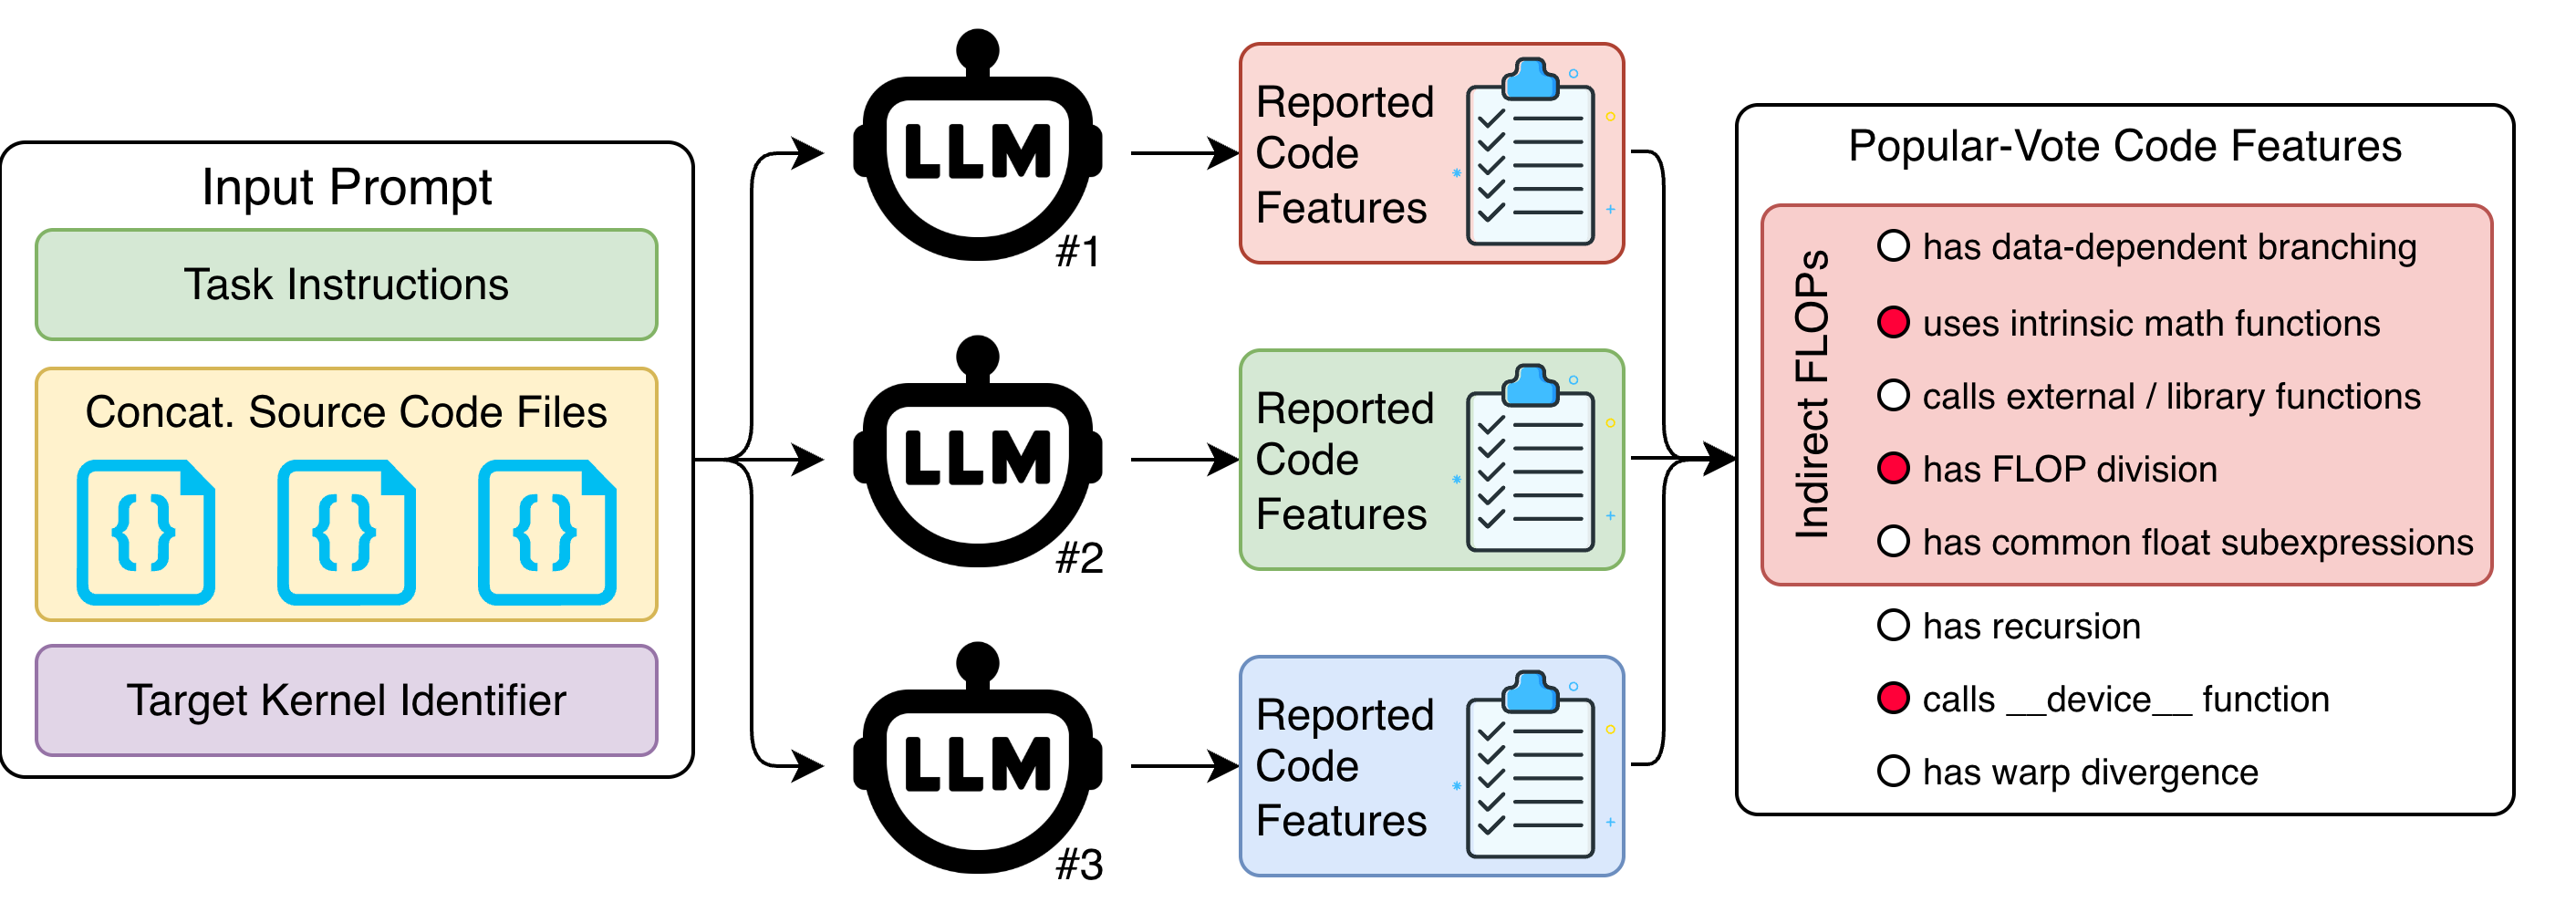
\includegraphics[width=0.98\linewidth]{figures/codeFeatureVoting.drawio.png}
    %\caption{We use an LLM-based voting scheme to categorize the code features present in each kernel. This allows us to classify the CUDA/OpenMP kernels in our dataset according to source-level features that can produce additional \textit{hidden} FLOP operations, often only becoming apparent post-compilation.}
     \caption{Voting ensemble used to label error-prone source features. Four inexpensive LLMs each vote three times per kernel, and a feature is marked present if it receives a majority of the 12 votes.}
    \label{fig:llmVotingScheme}
\end{figure}


\textbf{Evaluation Metrics.}
% Our goal is to evaluate how well current SoTA LLMs predict GPU kernel arithmetic intensity.
% We do so from two complementary perspectives: \textbf{(a)} quantitative \rai error and \textbf{(b)} binary Roofline-class agreement.
% Perspective \textbf{(a)} measures how closely the predicted \rai matches the expected \rai derived from profiling, while perspective \textbf{(b)} asks whether the model correctly identifies a kernel as bandwidth-bound or compute-bound.
% The second perspective is useful because even imperfect \rai estimates may still preserve the optimization-relevant bound classification.
We evaluate the LLMs from two complementary perspectives: \textbf{(a)} quantitative \rai error and \textbf{(b)} binary Roofline-class agreement.
The first measures numerical accuracy against the profiled \rai, while the second asks whether the model preserves the optimization-relevant bound classification.

For perspective \textbf{(a)}, we compute a percent prediction error for each \rai prediction at each FLOP precision.
Given a FLOP precision $\texttt{FPXX} \in \{\texttt{FP16}, \texttt{FP32}, \texttt{FP64}\}$, we compute the percent error as follows:
\[
\text{\% error}_{\texttt{FPXX}} = 100\frac{\text{predicted}_{\texttt{FPXX}} - \text{expected}_{\texttt{FPXX}}}{\text{expected}_{\texttt{FPXX}}}.
\]
% We note that this metric is bounded from the left, as a minimum of -100\% because the smallest prediction value is 0.
% Values less than 0\% are considered under-predictions, while values above 0 are considered over-preditions.
This metric is left-bounded at -100\%, with negative values denoting under-prediction and positive values denoting over-prediction.

For perspective \textbf{(b)}, we compare the predicted and expected binary bound classes using the GPU-specific balance points listed in \autoref{tab:gpu_specs}: a kernel is classified as compute-bound when its \rai exceeds the relevant balance point, and bandwidth-bound otherwise.
Together, these two views measure both numerical error and whether the model preserves the higher-level performance conclusion that would guide optimization effort.



\textbf{Code Feature Error Correlation}
% To measure how strongly each code feature is associated with \rai prediction error, we use \emph{Cliff's Delta}, a nonparametric effect-size measure comparing samples in which a feature is present against samples in which it is absent. 
% For a given feature $f$, let $E_f^{+}$ be the set of absolute \rai prediction errors for samples where $f$ is present, and let $E_f^{-}$ be the set of absolute \rai prediction errors for samples where $f$ is absent. 
To measure how strongly each code feature is associated with \rai prediction error, we use \emph{Cliff's Delta}, a nonparametric effect-size measure comparing feature-present and feature-absent samples.
For a given feature $f$, let $E_f^{+}$ and $E_f^{-}$ denote the sets of absolute \rai prediction errors for samples where $f$ is present and absent, respectively.
Cliff's Delta is defined as

\[
\delta_f
=
\frac{\#(x > y) - \#(x < y)}
{|E_f^{+}| \cdot |E_f^{-}|},
\qquad x \in E_f^{+},\; y \in E_f^{-},
\]

where $\#(x > y)$ counts the number of pairwise comparisons in which the feature-present \textit{absolute} \rai error exceeds the feature-absent \textit{absolute} \rai error, and $\#(x < y)$ counts the number of comparisons in which it is smaller.

The value of $\delta_f$ lies in $[-1,1]$. A value of $\delta_f = 1$ means that every feature-present sample has larger \rai error than every feature-absent sample; $\delta_f = -1$ means the opposite; and $\delta_f = 0$ indicates that neither group consistently dominates the other. 
Thus, positive values indicate that the presence of feature $f$ is associated with higher \rai prediction error, whereas negative values indicate that feature-present kernels tend to have lower \rai error.

We use Cliff's delta because our problem compares a binary predictor (code feature present versus absent) against a continuous error quantity whose distribution is often skewed and may contain outliers. 
Intuitively, if a feature such as ``\textit{Has FLOP Division}'' has $\delta_f = 0.58$, this means that, across all present-versus-absent pairwise comparisons, the FLOP division cases more often have larger \rai error than the non-division cases. 

% In this setting, a rank-based effect size is more informative than a significance test alone, since our goal is to identify which kernel features are most strongly associated with \rai misprediction and in which direction. 



















\section{Evaluation}
\label{sec:evaluation}

This section evaluates whether off-the-shelf LLMs can act as useful Roofline triage tools for GPU kernels by predicting runtime \rai from static code features.
We compare two prompting settings used in the paper: \textit{source-only} and \textit{source+SASS}, where the former only provides pre-compilation information to make predictions, while the latter provide post-compilation SASS instructions corresponding to the target kernel of interest for prediction.
We focus on three LLMs in this evaluation, \gptfivefour, \gptoss, and \opus.
Due to the expensive query costs associated with the \gptfivefour and \opus LLMs, we only perform \rai predictions once for each kernel across all four target GPUs.
Given the large number ($254*4=1016$) of GPU-kernel combinations that we sample for each LLM, we are able to get a sufficient understanding of their overall performance.
% Because the \rai-percent-error distributions contain extreme outliers, we emphasize medians, interquartile behavior, and balanced classification accuracy rather than prediction means.
% \textit{Unless otherwise stated, the figures below are all based on predicting the \rai of kernels with a \textbf{non-zero expected \rai value}; this prevents skewing the data towards low \rai errors by kernels that do not perform any FLOP work or DRAM reads/writes.}
% We later perform an analysis including all kernels, regardless of \rai value.
Given the heavy-tailed \rai-percent-error distributions, we emphasize medians, interquartile behavior, and balanced classification accuracy.
\textit{Unless otherwise stated, the figures below only include kernels with non-zero expected \rai values; we later analyze all kernels, including zero-\rai cases.}



\begin{figure}[h]
    \centering
    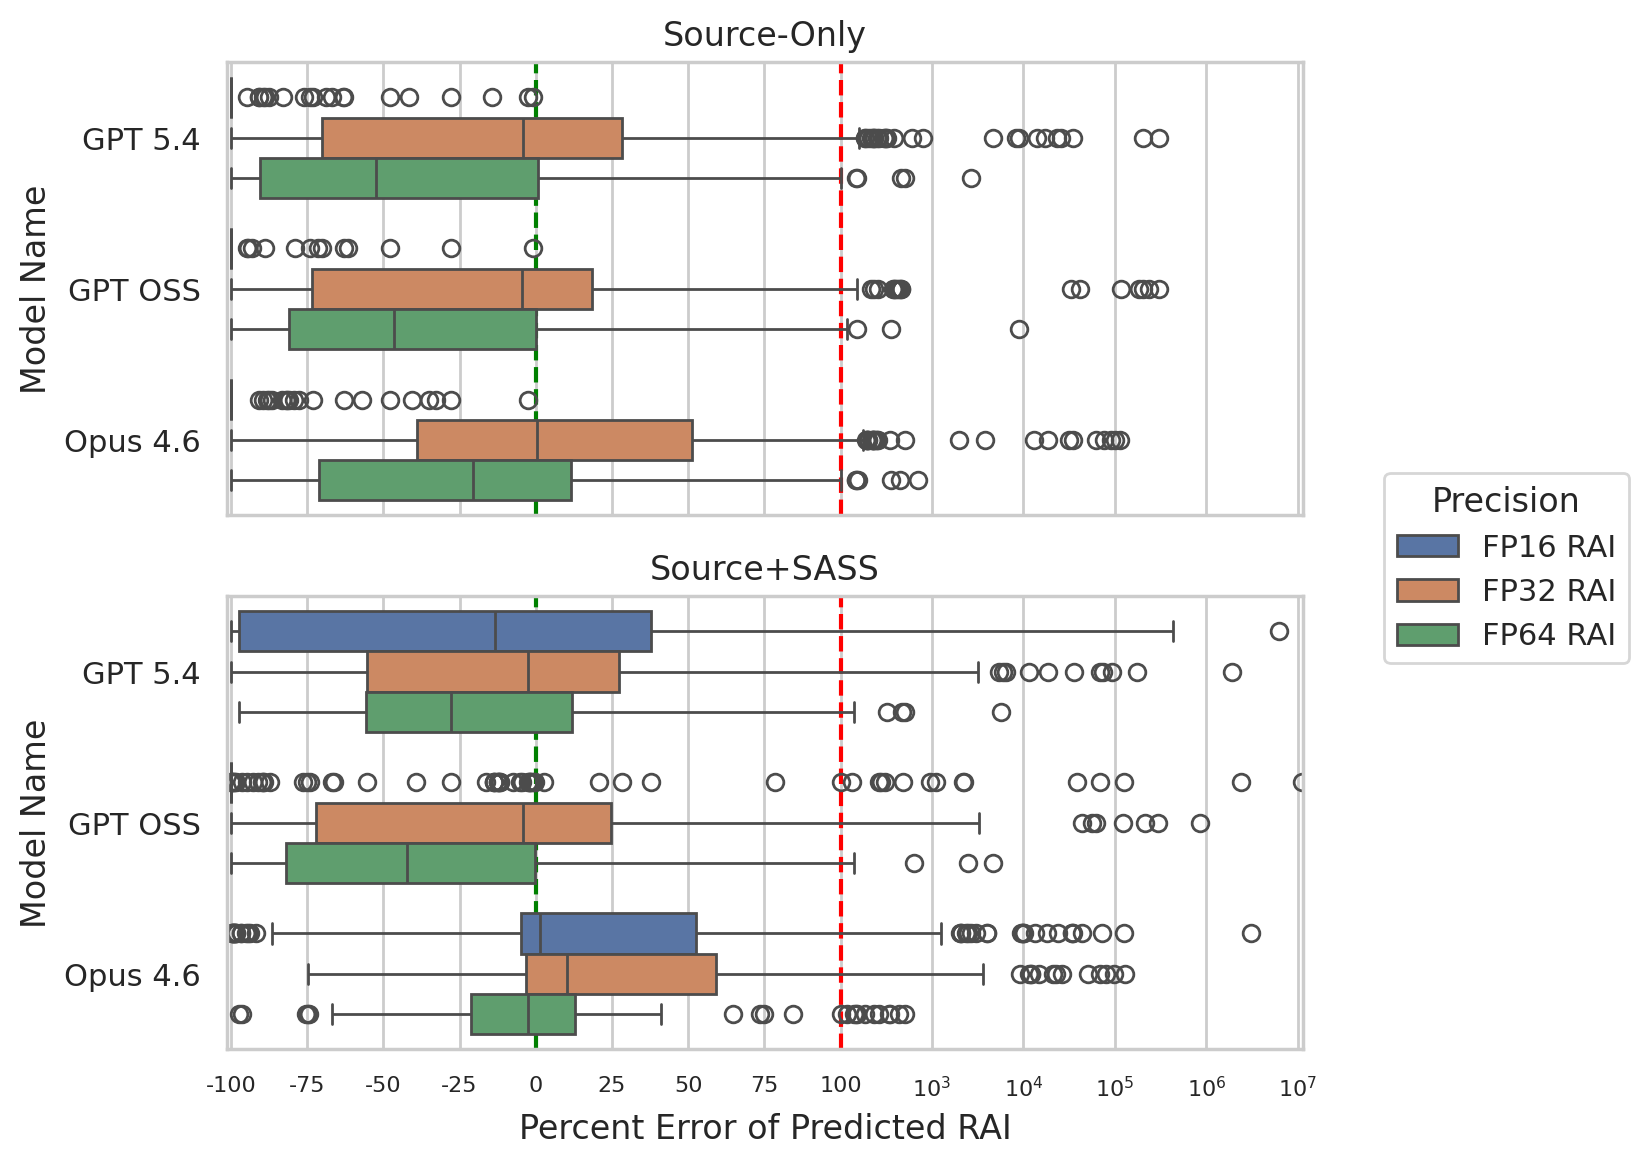
\includegraphics[width=0.95\linewidth]{figures/figure11_ai_percent_difference_boxplots.png}
    \caption{Distribution of \rai percent error for non-zero ground-truth cases, grouped by model and prompt setting across FP16/32/64 predictions.
    The hybrid linear-log x-axis expands the $\pm 100\%$ region while retaining large outliers; values closer to 0 are better.
    Adding post-compilation information helps the stronger models most, especially for FP16.}
    %\caption{Distribution of \rai percent error grouped by prompt type (top/bottom) and model (y-axis) across FP16, FP32, and FP64.
    %A hybrid linear-log scale emphasizes errors within $\pm 100\%$ while still showing larger outliers aggregated across all four GPUs and both runtimes.
    %}
    % \caption{Distribution of \rai percent error grouped by prompt type (top/bottom subplots) and model name (y-axis) across the three FLOP precisions (legend).
    % The plot is on a hybrid linear-log scale to emphasize the percent errors between $\pm 100\%$ in a linear scale, with errors beyond 100\% (the vertical red dashed indicator line) appearing on the log scale.
    % The errors shown for each model are aggregated from the predictions done on all four GPUs for both CUDA and OpenMP codes; this gives us a high-level view of the per-model prediction errors.
    % }
    \label{fig:per_model_ai_percent_diffs}
\end{figure}

\textbf{Per-Model \& Prompt Type Prediction Error.}
\autoref{fig:per_model_ai_percent_diffs} is a box-and-whisker visualization of the \rai percent prediction error for each FLOP precision and prompt type across the three tested LLMs: \gptfivefour, \gptoss, and \opus. 

There are a few trends to note:
\textbf{(1)} The FP16-\rai prediction error significantly improves for \gptfivefour and \opus when the SASS instructions are introduced.
From a median of -100\% on both, to a median of -13.5\% and 1.24\%, respectively.
\textbf{(2)} Unfortunately, the \gptoss model does not appear to make much use of the extra SASS information, given that it's median error stays at -100\% for FP16-\rai predictions, meanwhile it's FP32 and FP64 IQRs stay mostly the same.
\textbf{(3)} The cheap \gptoss and expensive \gptfivefour have very similar prediction distributions when given \sourceonly prompts, suggesting that in cases where a user can not get the SASS instructions for their kernel, the \gptoss model is a cost-effective alternative to querying \gptfivefour.
\textbf{(4)} Overall, the best performing model is \opus when prompted with \sourceSASS due to it's tighter IQRs and lower medians across all three FLOP precisions.

Given that the \gptoss model has a high chance of skewing model-aggregate metrics towards appearing more error-prone, we refer to \autoref{tab:nz_rai_results} to discuss the per-GPU and per-runtime prediction errors.
\autoref{tab:nz_rai_results} shows a heatmap of the proportion of non-zero \rai kernels that were predicted within a \pmten and \pmfifty \rai prediction error, where the \pmten acts as a strict error-bound and \pmfifty a more relaxed error-bound that allow us to better understand how well each LLM predicts \rai for each GPU, runtime, and prompt-type combination.
For \autoref{tab:nz_rai_results} we note that on the 3080 and A10 GPUs, the sampled OpenMP kernels did not perform any FP16 instructions, thus those metrics in the table are omitted.


% \autoref{fig:eval_ai_diff_by_model} is a box-and-whisker visualization of the \rai prediction error for each FLOP precision type across three tested LLMs: \opus, \gptoss, and \gptfivefour.
% The plot is on a log scale to more clearly show the prediction errors (predicted minus expected \rai), with the green vertical dashed line indicating an error of 0, while the red dashed lines indicate an error of +/-1.
% The top subplot shows the prediction errors when prompting only with source, while the bottom subplot prompts with source and SASS information.
% The errors shown for each model are aggregated from the predictions done on all four GPUs.
% 
% There are few major trends of note:
% (1) From the IQRs of each boxplot, roughly 50\% of all \rai predictions are within a +/-1 error away from the ground-truth profiled \rai.
% FP32-\rai (orange boxes) having the lowest overall prediction errors, followed by FP64-\rai (green boxes).
% (2) FP16-\rai (blue boxes) is always under-predicted from the \sourceonly setting, where the introduction of SASS instructions greatly ameliorates mispredictions.
% (3) The cheap \gptoss and expensive \gptfivefour have very similar prediction distributions in the \sourceonly setting, yet \gptoss fails to adequately use the post-compilation information in the \sourceSASS setting to improve the FP16-\rai error, given by it's FP16-\rai IQR still in the negative on the \sourceSASS prompts.

% Although the expensive models perform well in the \rai prediction task for many codes, there still exist many outlier cases with severe over- and under-prediction. 
% In the case of FP64-\rai predictions, given how the balance points listed in \autoref{tab:gpu_specs} range from 0.6 to 10, an \rai misprediction over or under by 1 could be the difference between a correct compute- or bandwidth-bound classification.
% We discuss this further in the next subsection. 

\input{listings/percent_summary_table}


% \begin{figure}[t!]
%     \centering
%     
\includegraphics[width=0.9\linewidth]{figures/figure1_ai_difference_boxplots.png}
%     \caption{Distribution of predicted minus expected Roofline Arithmetic Intensity, grouped by model and split into source-only and source+SASS settings. Separate boxes correspond to FP16, FP32, and FP64, and the dashed line marks zero error.}
%     \label{fig:eval_ai_diff_by_model}
% \end{figure}




% \begin{figure}[h!]
%     \centering
%     
\includegraphics[width=0.9\linewidth]{figures/figure3_ai_difference_boxplots_by_gpu.png}
%     \caption{Distribution of predicted minus expected arithmetic intensity grouped by target GPU and split into source-only and source+SASS settings.}
%     \label{fig:eval_ai_diff_by_gpu}
% \end{figure}

\textbf{Per-Runtime Prediction Error.}
In considering the CUDA/OpenMP runtime prediction errors, \autoref{tab:nz_rai_results} shows a few general trends:
\textbf{(1)} When making \sourceonly predictions with the OpenMP runtime, all the models struggle to make FP16-\rai predictions, given by the zero proportion of kernels that are predicted within the \pmfifty error range.
When it comes to the CUDA runtime under the same \sourceonly FP16-\rai conditions, the LLMs still struggle across all GPUs, but at the very least tease out a couple of close \rai estimates due to the non-zero \pmfifty error ranges.
This aligns with the fact that FP16 instructions often get inserted post-compilation, where prompting with \sourceSASS makes the instructions more apparent.
\textbf{(2)} If a choice needed to be made between using LLMs to predict on a CUDA or an OpenMP runtime, said choice is dependent on LLM model and FLOP precision of the target kernel.
Across GPUs, \opus is better at predicting FP32-based CUDA kernels because an average of 73.6\% of CUDA kernels have at most a \pmfifty error, while an average 66.1\% of OpenMP kernels have at most a \pmfifty error.
We see a similar trend for \gptfivefour, in favoring CUDA for FP32-based kernels.
As for FP64-based kernels, \opus does about the same on either runtime, where \gptfivefour does better for OpenMP codes.
\textbf{(3)} If LLM query budget is a consideration, the \gptoss model exhibits the same trend as its more recent \gptfivefour, where it's better at predicting FP64-based OpenMP codes, and FP32-based CUDA codes.

From these results, the general rule-of-thumb would be that the LLMs will give better predictions on CUDA codes that are FP16/FP32-heavy, and better predictions on OpenMP codes that are more FP64-heavy.


\textbf{Per-GPU Prediction Error.}
From the perspective of per-gpu error, \autoref{tab:nz_rai_results} shows that prediction error is not the same across GPUs, with A100 and H100 predictions being the most accurate when made by the \opus and \gptfivefour models.
For FP32-\rai predictions, the LLMs tend to predict the worst on the A10 GPU across both runtimes and prompt types, evidenced by how at best 15.7\% of the kernels have a \pmten error when predicted by \opus, however this misprediction effect seems to peter out at the \pmfifty error range, with the proportion of A10 kernels more closely matching the other GPUs.
These results align with the fact that that the 3080 and A10 GPUs have smaller 5MB and 6MB L2 cache sizes, respectively, therefore the LLMs have to account for L2 cache misses serviced by GPU DRAM---implying higher DRAM Bytes read---which can easily throw off the denominator of the \rai calculation.
In the A100 and H100 with larger 40MB and 50MB L2 caches, respectively, the LLMs can more correctly assume that total DRAM writes end up being small because the working set of memory is more likely to stay in the L2 cache. 
The takeaway here is that LLMs still struggle to accurately account for caching effects that impact the memory traffic on GPUs with smaller caches, thus leading to worse predictions.
If possible, LLM-based \rai predictions should be done on GPUs with larger caches for less error-prone results.

% For FP64-\rai predictions, the \pmten proportion is lower across the board in comparison to the FP32-\rai, however when we consider the more relaxed \pmfifty error, we see a larger proportion of predictions (often 10-20\% more) 
% \autoref{fig:eval_ai_diff_by_gpu} shows the same \rai error metric as \autoref{fig:eval_ai_diff_by_model}, however it is broken down by GPU model and is an aggregate across all three LLMs.
% We can again notice that about 50\% of the predictions are within a small +/-1 error range for the more straight-forward FP32 and FP64 predictions, however when doing \sourceonly predictions, the FP16 errors (blue boxes) are much larger, where the LLMs are severely undercounting across all architectures.
% This is primarily due to how the compiler inserts more FP16 ops into the A100 and H100 kernels, which only becomes apparent upon inspection of SASS.
% The introduction of SASS improves predictions across the A100 and H100 GPUs, primarily because it makes abundantly clear to the LLMs the quantity of FP16 instructions that get compiled into the program.
% An unexpected result is how the \sourceSASS configuration doesn't improve the FP64 predictions (green boxes) by much across 




% \autoref{fig:eval_ai_diff_by_runtime} shows the same box-and-whisker error data split by CUDA and OpenMP runtime, aggregated over the LLM models and GPU archs.
% There are two major points that should be highlighted:
% \begin{enumerate}
%     \item For either runtime, the prediction errors are quite similar, indicating that current LLMs can handle reasoning about either runtime just as equally.
%     \item The inclusion of SASS lowers the error of FP16-\rai predictions for both runtimes, pushing the IQR into the +/-1 error band.
% \end{enumerate}
% As for the FP64 and FP32 errors, there is not too much of a difference.


% \begin{figure}
%     \centering
%     
\includegraphics[width=0.9\linewidth]{figures/figure4_ai_difference_boxplots_by_runtime.png}
%     \caption{Distribution of predicted minus expected arithmetic intensity grouped by runtime (CUDA versus OpenMP) and split into source-only and source+SASS settings.}
%     \label{fig:eval_ai_diff_by_runtime}
% \end{figure}


\begin{figure}[t!]
    \centering
    %
\includegraphics[width=0.9\linewidth]{figures/figure2_ai_bound_confusion_heatmaps.png}
    %\caption{Confusion heatmaps comparing expected and predicted \rai bound class: Compute-Bound (CB) and Bandwidth-Bound (BB). 
    %Each cell is annotated with FP16, FP32, and FP64 code percentages corresponding to the proportion of kernels that were expected to be a part of a bound-class that were predicted in another bound-class; intuitively, darker main-diagonal cells indicate stronger agreement between expected and predicted Roofline class.}

    
\includegraphics[width=0.95\linewidth]{figures/figure2_5_ai_bound_confusion_heatmaps_with_zero.png}
    \caption{Confusion heatmaps for the three \rai classes used in the paper: zero-valued, compute-bound, and bandwidth-bound.
    Subplot rows correspond to models and columns to prompt settings; each cell reports FP16, FP32, and FP64 percentages for that expected-versus-predicted class pair.
    Darker diagonal cells indicate stronger agreement. 
    Post-compilation information most clearly improves compute-bound and bandwidth-bound classification for the stronger models.}
    %\caption{Confusion heatmaps comparing the expected and predicted \rai classification accuracy: Zero-value, Compute-Bound (\compbound), and Bandwidth-Bound (\bandbound).
    %Each cell is annotated with FP16, FP32, and FP64 code percentages corresponding to the proportion of kernels that were predicted to be a part of a particular classification. 
    %Each subplot row corresponds to a particular LLM, while each subplot column corresponds to prompting \sourceonly or with \sourceSASS.
    %Intuitively, darker main-diagonal cells indicate stronger agreement between expected and predicted \rai classifications.
    %}
    \label{fig:eval_ai_bound_heatmaps}
\end{figure}


%%% Need to change this plot to include the zero cases

\textbf{\rai Classification Accuracy.}
% The previously-discussed results focused on the predictions made for the kernels with non-zero expected \rai values.
% We now shift our focus to study both zero and non-zero expected-value \rai kernels; we do so from the perspective of correct binary Roofline classification accuracy.
We now extend the analysis to both zero and non-zero expected-value \rai kernels by evaluating Roofline classification accuracy.
The benefit of this perspective is that although a large number of \rai predictions may have a large percent error of \pmfifty, if they are on the correct side of each GPU Roofline's balance point, they will be considered correctly classified as either Bandwidth-Bound (\bandbound, less than balance point) or Compute-Bound (\compbound, greater than balance point).
Having a correct classification can dramatically change the types of optimizations applied to a kernel during tuning; if \compbound, the optimizer may focus on doing more FLOP work for each byte of memory moved, and if \bandbound, coalescing memory movement for each FLOP performed).
There exists a third \rai classification: we consider a \rai value of \textit{zero} its own class so as not to skew the \bandbound accuracy results.
% Given that a \rai prediction error falls within the +/-1 range for about 50\% of the tested codes, we consider how this affects the \rai classification of a kernel as being Bandwidth-Bound (\bandbound) or Compute-Bound (\compbound).
\autoref{fig:eval_ai_bound_heatmaps} depicts the classification accuracy of the predicted \rai results, where the confusion tables show the percent of cases that were predicted as zero-valued, \bandbound, or \compbound across all three models (rows) when they were prompted with \sourceonly or with \sourceSASS (columns). 
From the figure we can note a few points:
\textbf{(1)} Prompting on all three models with \sourceonly inputs, causes many \bandbound and \compbound kernels to be misclassified as having 0 FP16-\rai. 
This effect is consistent with the previous results in \autoref{tab:nz_rai_results} and \autoref{fig:per_model_ai_percent_diffs}.
The prediction accuracies in all the cells are very similar between LLMs with \sourceonly prompting, implying that if a user does not have SASS instructions to add to their prompt, they can get similar \rai classification results from both the economical and premium LLMs.
\textbf{(2)} Another repeat trend is how prompting with \sourceSASS significantly improves correct prediction accuracy across LLMs, with \opus seeing the best improvements in accuracy of 95\% or greater for the \compbound and \bandbound kernels.
% \textbf{(3)} Across all models and prompt types, the Zero-class classification is frequently correct, scoring consistently-high accuracies.
% Unfortunately, when we prompt with \sourceSASS, all the models begin to incorrectly classify 5-15\% more of the Zero-class FP32 kernels as \bandbound.
% We found this effect was due to X.

The takeaway here is that across all three LLMs, \textbf{(a)} with simple \sourceonly prompting, a fiscally-conscious user may stick to \gptoss for \rai classifications, and \textbf{(b)} the inclusion of SASS instructions improves classification accuracy for the expensive LLMs, especially on \compbound kernels.
% This is a common trend of ``\textit{you-get-what-you-paid-for}'', where the classification accuracy directly improves from cheapest to most expensive LLM.

%Across all models, the inclusion of SASS improves the FP16 CB prediction accuracy significantly.
%In the cases of \opus and \gptfivefour, they go from 100\% misprediction to 100\% and 76\% correct predictions respectively.
%Unfortunately, in the case of \gptoss, the improvements are meager, and can even cause a drop in accuracy as seen for the FP64 case. 





\textbf{Error-Prone Code Features.}
\autoref{fig:codeFeatureAssociationHeatmap} shows a \rai prediction error attribution heatmap split by prompt-type and LLM model, using the Cliff's Delta metric defined at the end of \autoref{sec:methodology}.
For this error analysis, we purposely include the kernels that were predicted on with expected \rai values of zero, as the Cliff's Delta metric is robust to skewness.
For reference, the different categories of code feature flags are described in more detail in Appendix \autoref{sec:codeFeatureCategoriesAppendix}.

What we end up finding is that across both runtimes, prompt types, and GPU types, the largest chances of \rai mispredictions occur when FLOP division, FLOP subexpressions, special FLOP math functions, and loop-invariant FLOPs are present.
FLOP division introduces not only new FLOPs into the SASS, but also data-dependent branching to implement the Newton-Raphson root-finding approach used in the IEEE FLOP division spec \cite{IEEEStandardFloatingPoint2019}. 
Similarly, \textit{special} (i.e.: transcendental) math functions like \texttt{sin} and \texttt{cos} also introduce new FLOPs into the SASS that the LLMs much account for.
On the other hand, \textit{common FLOP subexpression elimination} and \textit{loop-invariant FLOP hoisting} remove repeat operations from the SASS, easily allowing an LLM to overcount repeat work during static analysis.
Given the very direct influence these features have on the final number of floating point operations that get included into a kernel's instructions, it makes sense that they can lead to the highest misprediction errors.

On the other end of the spectrum, the features of \textit{deterministic grid/block size} detect whether the grid and block size can be statically determined via constant propagation of literals, macros, and command-line arguments supplied during prompting.
\autoref{fig:codeFeatureAssociationHeatmap} show that across all cases, these two features tend to lean towards the negative Cliff Delta values, yet hang around 0, indicating that there are only slightly more cases where the presence of these features has a lower \rai error than without.

The takeaway from this analysis is that \textbf{(a)} regardless of LLM and prompt-type, the same code features contribute to the most (and least) \rai prediction errors, and \textbf{(b)} users should try to minimize the occurrence of FLOP divison, subexpressions, special math functions, and loop-invariant ops to maximize the chances of correct LLM-based \rai predictions; similarly, maximizing the ease with which an LLM could determine grid/block size can aid in accurate predictions.

% This intuitively makes sense, as being able to correctly determine the grid and block sizes leads to proper thread count prediction, allowing for accurate FLOP and DRAM read/write count predictions.

% \autoref{fig:promptFeatureAssociationHeatmap} and \autoref{fig:gpuFeatureAssociationHeatmap} show a \rai prediction error attribution heatmap split by prompt type and GPU, respectively, for each runtime, using the Cliff's Delta metric defined at the end of \autoref{sec:methodology}. 
% For this error analysis, we purposely include the kernels that were predicted on with expected \rai values of 0, as the Cliff's Delta metric is robust to skewness.
% For reference, the different categories of code feature flags are described in more detail in Appendix \autoref{sec:codeFeatureCategoriesAppendix}.
% 
% What we end up finding is that across both runtimes, prompt types, and GPU types, the largest chances of \rai misprediction occur when FLOP division, FLOP subexpressions, special FLOP math functions, and loop-invariant FLOPs are present.
% FLOP division introduces not only new FLOPs into the SASS, but also data-dependent branching to implement the Newton-Raphson root-finding approach used in the IEEE FLOP division spec \cite{IEEEStandardFloatingPoint2019}. 
% Similarly, \textit{special} (i.e.: transcendental) math functions like \texttt{sin} and \texttt{cos} also introduce new FLOPs into the SASS that the LLMs much account for.
% On the other hand, \textit{common FLOP subexpression elimination} and \textit{loop-invariant FLOP hoisting} remove repeat operations from the SASS, easily allowing an LLM to overcount repeat work during static analysis.
% Given the very direct influence these features have on the final number of floating point operations that get included into a kernel's instructions, it makes sense they can lead to the highest misprediction errors.
% 
% One of the most salient distinctions that can be made from these plots is how the presence of \textit{calls to helper functions} (i.e.: calling a \texttt{\_\_device\_\_} function in CUDA, or a plain function call in an OpenMP parallel region), introduces much less errors for CUDA codes than for OpenMP.
% It turns out that this is caused by TODO.
% This outcome aligns with how \cite{timeMattisonPaperwithOpenMPStudy} found that OpenMP is less present in LLM training data (re-write this sentence).

% Lastly, the features of \textit{deterministic grid/block size} detect whether the grid and block size can be statically determined via constant propagation of literals, macros, and command-line arguments supplied during prompting.
% \autoref{fig:promptFeatureAssociationHeatmap} and \autoref{fig:gpuFeatureAssociationHeatmap} show that across all cases, these two features tend to lean towards the negative Cliff Delta values, yet hang around 0, indicating that there there are only slightly more cases where the presence of these features has a lower \rai error than without.
% This intuitively makes sense, as being able to correctly determine the grid and block sizes leads to proper thread count prediction, allowing for accurate FLOP and DRAM read/write count predictions.

\begin{figure}
    \centering
    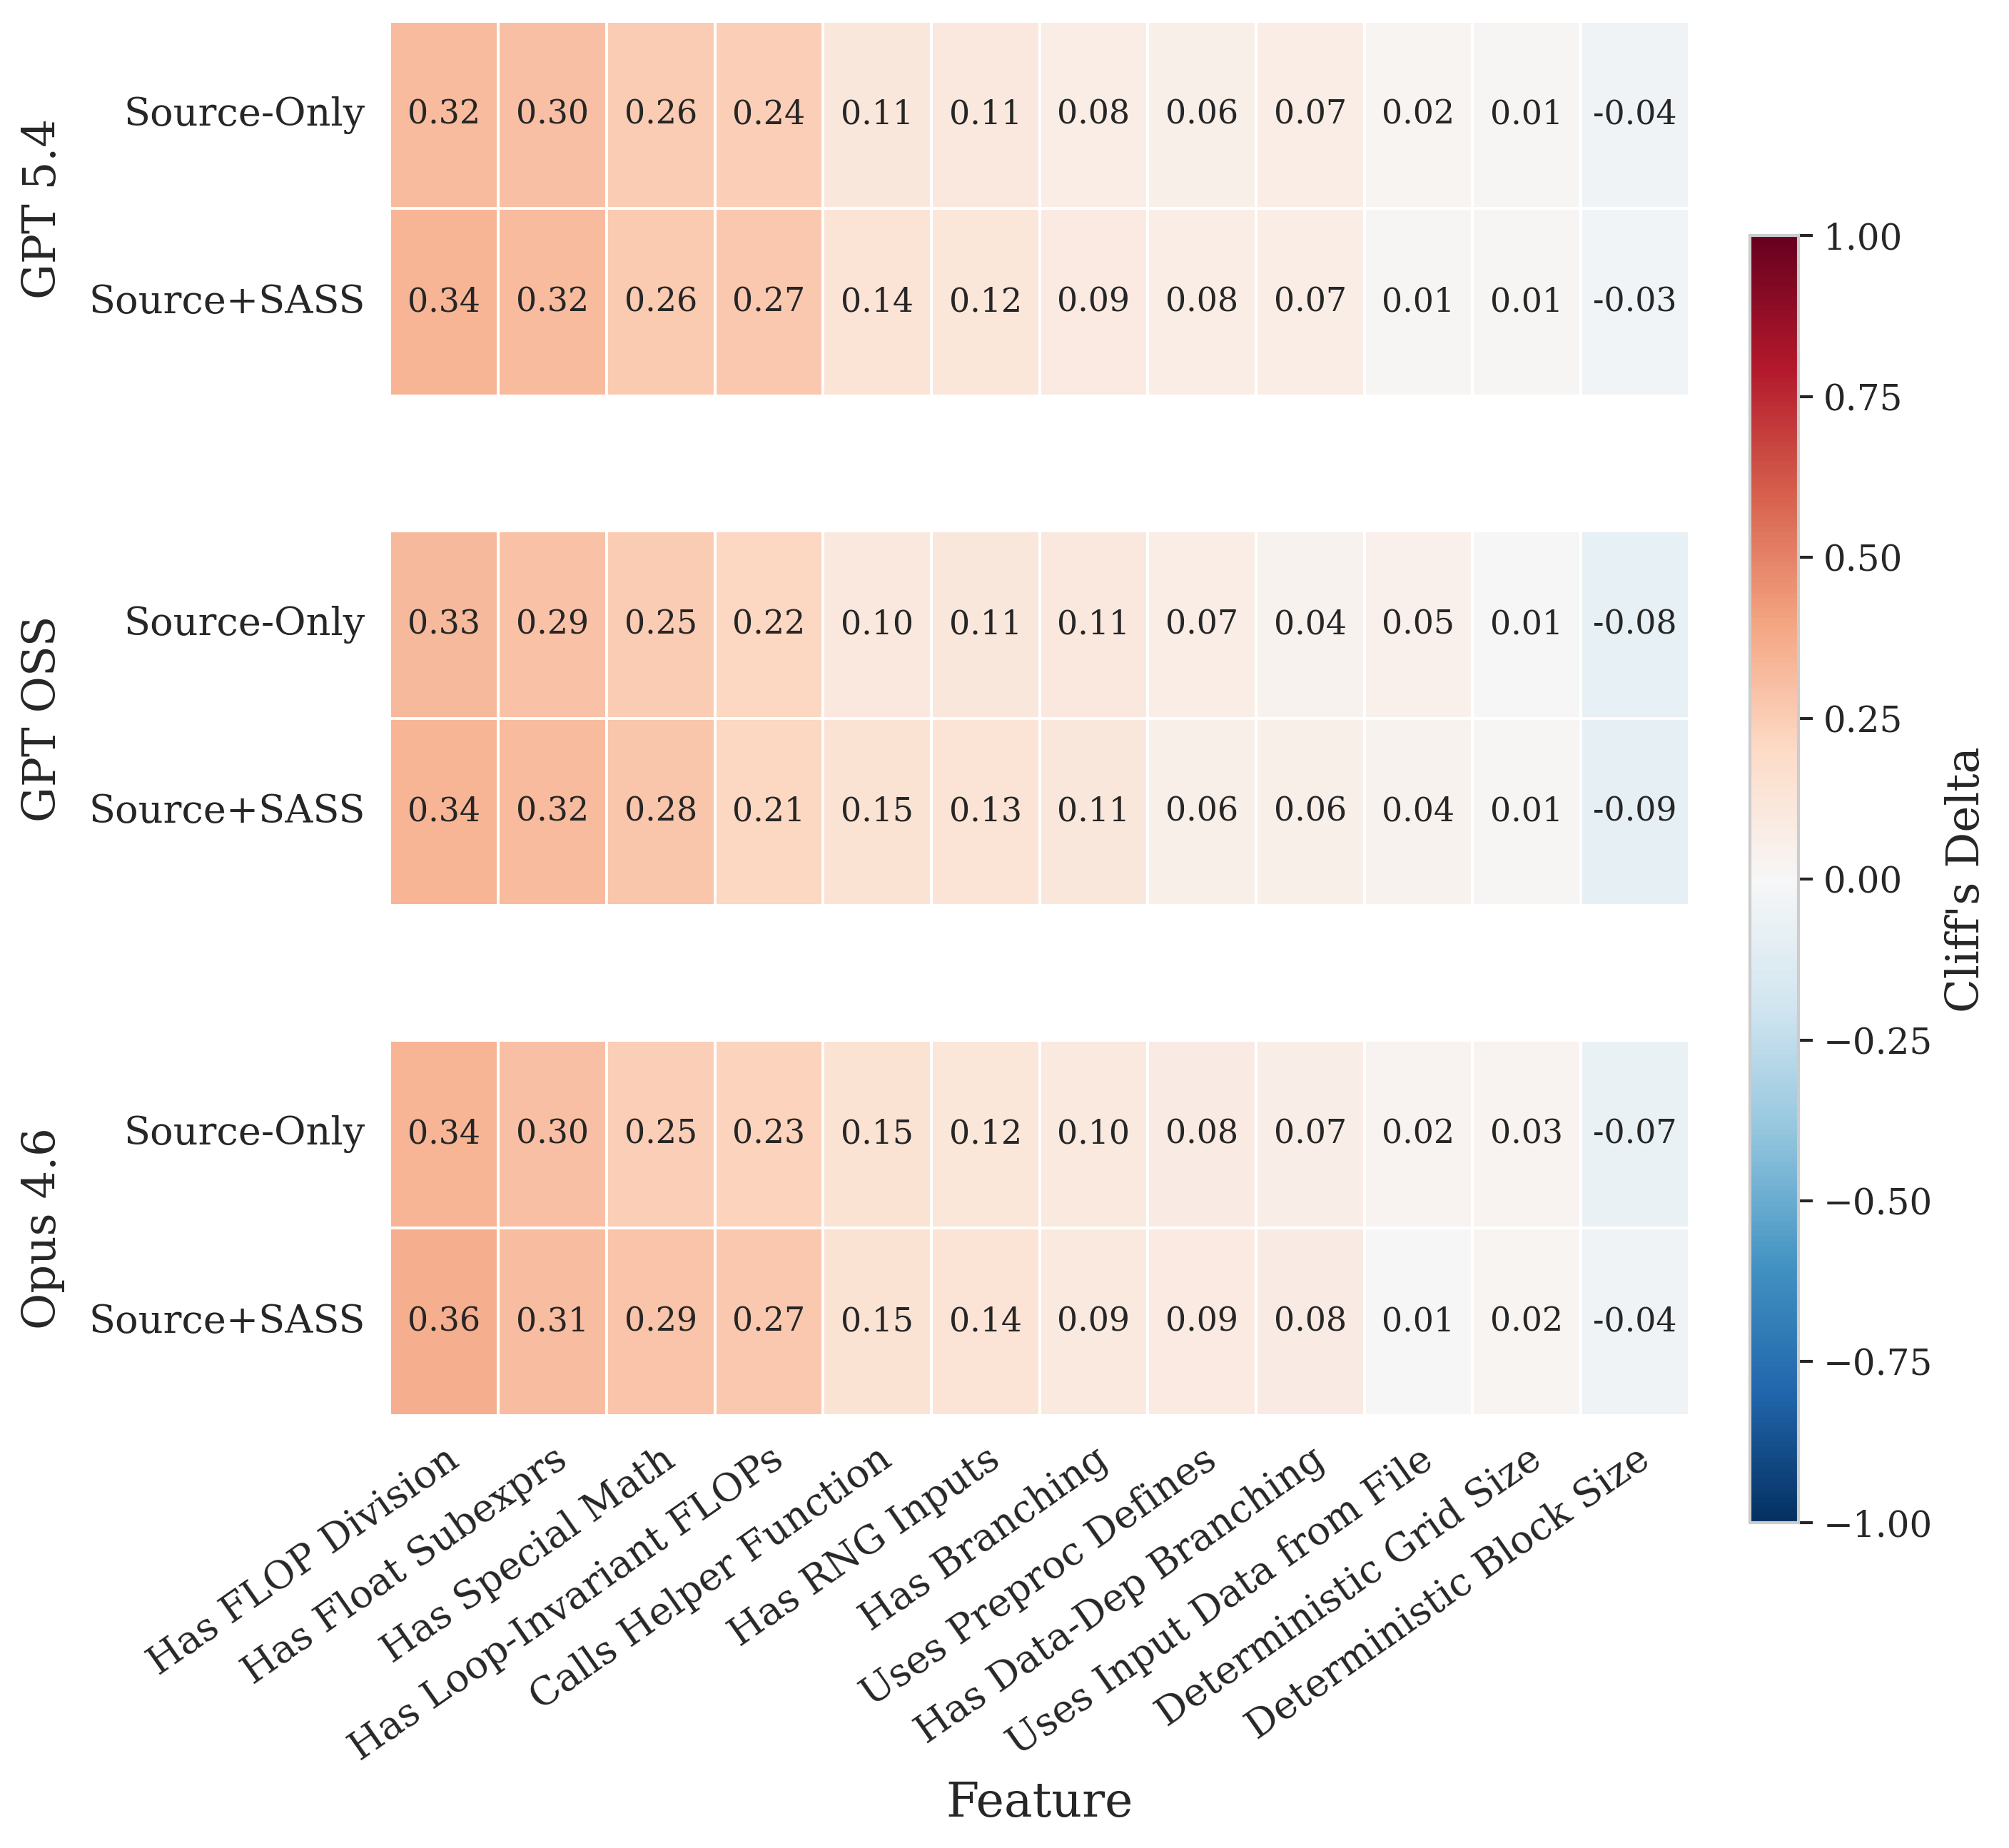
\includegraphics[width=0.95\linewidth]{figures/figure1_model_feature_association_heatmap.png}
    \caption{Cliff's Delta heatmap relating source features to absolute \rai error, split by prompt type and model. 
    Positive values mean the feature is associated with larger errors, negative values with smaller errors.
    FLOP division, reusable subexpressions, special math functions, and loop-invariant work are the most consistent error drivers.}
     %\caption{Code feature error attribution heatmap split by prompt type and model name.
     %Errors are consistent across models and prompt types, with the presence of \textit{FLOP division} and \textit{float subexpressions} leading to a higher chance of \rai mispredictions.}
    \label{fig:codeFeatureAssociationHeatmap}
\end{figure}

% \begin{figure}
%     \centering
%     
\includegraphics[width=0.95\linewidth]{figures/runtime_feature_association_heatmap.png}
%     \caption{Code feature error attribution heatmap split by prompt type and runtime.
%     Errors are similar across both prompting types, with the presence of \textit{FLOP division} and \textit{float subexpressions} leading to a higher chance of \rai mispredictions.}
%     \label{fig:promptFeatureAssociationHeatmap}
% \end{figure}
% 
% \begin{figure}
%     \centering
%     
\includegraphics[width=0.95\linewidth]{figures/gpu_feature_association_heatmap.png}
%     \caption{Code feature error attribution heatmap split by GPU and runtime.
%     Errors are similar across all prompting types, with the presence of \textit{FLOP division} and \textit{float subexpressions} leading to a higher chance of \rai mispredictions.}
%     \label{fig:gpuFeatureAssociationHeatmap}
% \end{figure}








\textbf{LLM Cost and Time Analysis.}
\autoref{fig:costDistrib} shows query cost distributions (in USD) by model and prompt type.
We focus on distinguishing the costs between prompt types, as including SASS instructions increases the amount of tokens each LLM has to process, thus directly increasing cost.
\gptoss is by far the cheapest, with a median cost of \$0.001 per query and under \$3 for roughly 2000 queries.
\gptfivefour is next at \$0.020/\$0.031 median cost for \sourceonly/\sourceSASS, while \opus is highest at \$0.068/\$0.107 and about \$160 total.
This cost ranking closely matches predictive performance: \opus and \gptfivefour are more accurate, but far more expensive.
% \autoref{fig:costDistrib} shows the distribution of query costs (in USD) for each of the prompt types across the three sampled LLMs.
% The right-side margin shows the summed cost across all samples.
% The input/output query token costs are described in \autoref{tab:llm_comparison}, and set by the LLM providers.
% What we can notice is that the \gptoss model is incredibly cost-effective, with a median cost-per-query of \$0.001 for both \sourceonly and \sourceSASS prompting; only costing less than \$3 to make about 2000 queries.
% The next cheapest model is \gptfivefour, with a median cost of \$0.020 and \$0.031 for \sourceonly and \sourceSASS prompts, respectively; costing cumulatively \$47 to perform all the queries. 
% The most expensive is the \opus model, with median costs of \$0.068 and \$0.107 for \sourceonly and \sourceSASS, respectively; costing cumulatively \$160 for the same queries as the other models.
% This cost inequality aligns closely with the predictive performance of the models, where the most expensive (\opus and \gptfivefour) LLMs make better predictions than the cheaper/inaccurate \gptoss.

\begin{figure}[t!]
    \centering
    
\includegraphics[width=0.95\linewidth,trim=0 0 0 0.9cm,clip]{figures/plot3_cost_distribution.png}
    \caption{Per-query cost distribution by model and prompt setting.
    Totals across all queries are shown on the right; adding SASS usually increases cost, while the cheapest model remains orders of magnitude less expensive than the strongest models.}
    %\caption{Query cost distribution across LLMs and prompting type. 
    %Total cumulative costs are shown on the right margin.
    %The queries using \sourceSASS are often more expensive than those of \sourceonly.
    %The \gptoss model is extremely cost-effective in comparison to \gptfivefour and \opus.
    %}
    \label{fig:costDistrib}
\end{figure}

\autoref{fig:timeDistrib} shows the distribution of the query times (in seconds) for each of the prompt types across the three sampled LLMs.
This plot captures the LLM query response generation times, excluding HTTP request travel time.
Surprisingly, \gptfivefour has the lowest inference times, with a median around 10.9 and 12.0 seconds for \sourceonly and \sourceSASS prompting, respectively.
We note that the \gptoss model has the longest query times, with medians around 32.7 and 32.0 seconds for both prompt types, whereas \opus had median times around 21.9 and 29.3 seconds for \sourceonly and \sourceSASS, respectively.
We urge users to jointly consider the monetary, query time, and prediction accuracies of these models when deciding which to use.
Although the \gptoss model is inexpensive, it is not as fast or accurate in comparison to its more recent \gptfivefour counterpart which takes about a third of the time to query, but at about 20x the cost.

\begin{figure}[t!]
    \centering
    
\includegraphics[width=0.95\linewidth,trim=0 0 0 0.9cm,clip]{figures/plot2_query_time_distribution.png}
    \caption{Per-query response-time distribution by model and prompt setting, excluding HTTP latency.
    Adding SASS modestly increases latency for the stronger models, while \gptfivefour is the fastest overall, and \gptoss the slowest.}
    %\caption{Query time distribution across LLMs and prompting type.
    %Querying with or without SASS has little effect on the \gptoss model, however including SASS can cause a median query time increase of about 10\% and 30\% on \gptfivefour and \opus, respectively.}
    \label{fig:timeDistrib}
\end{figure}



%\subsection{RQ1: Generalization Across Architectures}
%
%RQ1 asks whether LLMs can predict arithmetic intensity accurately enough across multiple GPU architectures to remain useful as hardware-free triage tools.
%We answer this question from two perspectives introduced in \autoref{sec:methodology}: (1) quantitative AI error, measured as \textit{predicted AI} minus \textit{expected AI}, and (2) binary Roofline-class agreement, measured by whether the predicted and expected AI values place a kernel on the same side of the architecture-specific balance point.
%
%\autoref{fig:eval_ai_diff_by_model} summarizes the signed AI-error distributions for the two evaluated models under the source-only and source+SASS settings.
%Across both models, the \textbf{median signed FP32 AI error is already close to zero} in the source-only setting, but the tails are heavy, so median absolute AI error is the more stable summary.
%As shown in \autoref{tab:eval_model_summary}, Claude Opus 4.6 is consistently better than GPT-5.4 on quantitative AI prediction: under source-only prompting, its median absolute AI error is 0.321 for FP32 and 0.416 for FP64, compared to 0.746 and 0.590 for GPT-5.4.
%The same ranking holds in the source+SASS setting, where Claude has lower FP32 and FP64 median absolute AI error.
%
%\autoref{fig:eval_ai_bound_heatmaps} shows that \textbf{bound-class agreement is often stronger than raw AI accuracy would suggest}, especially for FP32.
%For source-only prompting, balanced accuracy on FP32 is already high for both models: 0.928 for Claude and 0.889 for GPT-5.4.
%FP64 is noticeably harder, dropping to 0.784 for Claude and 0.679 for GPT-5.4 under source-only prompting.
%FP16 is the clearest failure case for source-only prompting: both models achieve a balanced accuracy of 0.5 because they effectively predict the bandwidth-bound class only, even though raw accuracy remains high due to class imbalance.
%
%\autoref{fig:eval_ai_diff_by_gpu} further shows that generalization is not uniform across architectures.
%For FP32, source-only median absolute AI error ranges from 0.321 on A100 to 0.587 on the RTX 3080, suggesting reasonably stable behavior across GPUs despite large outliers.
%FP64 is more architecture-sensitive: source-only balanced accuracy is 0.788 on the RTX 3080, 0.677 on the A10, but falls to 0.5 on both A100 and H100, indicating that the models frequently miss the compute-bound cases on those architectures.
%Overall, these results suggest that off-the-shelf models are already useful for \textbf{FP32-oriented triage across architectures}, but their FP64 behavior is less reliable and remains strongly architecture-dependent.

% \begin{table*}[t]
%     \centering
%     \caption{Per-model summary of arithmetic-intensity error and bound-class agreement. We report median absolute \rai error because the signed \rai-error distributions are heavy-tailed.}
%     \label{tab:eval_model_summary}
%     \scriptsize
%     \setlength{\tabcolsep}{4pt}
%     \renewcommand{\arraystretch}{1.05}
%     \resizebox{\textwidth}{!}{%
%     \begin{tabular}{llcccccc}
%     \toprule
%     \textbf{Model} & \textbf{Setting} & \textbf{FP16 Med. $|\Delta \mathrm{AI}|$} & \textbf{FP32 Med. $|\Delta \mathrm{AI}|$} & \textbf{FP64 Med. $|\Delta \mathrm{AI}|$} & \textbf{FP16 Bal. Acc.} & \textbf{FP32 Bal. Acc.} & \textbf{FP64 Bal. Acc.} \\
%     \midrule
%     Claude Opus 4.6 & source-only  & 0.507 & 0.321 & 0.416 & 0.500 & 0.928 & 0.784 \\
%     Claude Opus 4.6 & source+SASS  & 0.056 & 0.305 & 0.204 & 0.975 & 0.958 & 0.779 \\
%     GPT-5.4         & source-only  & 0.512 & 0.746 & 0.590 & 0.500 & 0.889 & 0.679 \\
%     GPT-5.4         & source+SASS  & 0.341 & 0.640 & 0.534 & 0.849 & 0.890 & 0.726 \\
%     \bottomrule
%     \end{tabular}%
%     }
% \end{table*}





% \begin{table*}[t]
%     \centering
%     \caption{Architecture-level summary aggregated across both models. FP16 is omitted because the RTX 3080 and A10 contain very few nonzero-AI FP16 samples, making architecture-level comparisons less stable.}
%     \label{tab:eval_gpu_summary}
%     \scriptsize
%     \setlength{\tabcolsep}{4pt}
%     \renewcommand{\arraystretch}{1.05}
%     \resizebox{\textwidth}{!}{%
%     \begin{tabular}{lcccccccc}
%     \toprule
%     \textbf{GPU} & \textbf{FP32 Med. $|\Delta \mathrm{AI}|$} & \textbf{FP32 Med. $|\Delta \mathrm{AI}|$} & \textbf{FP64 Med. $|\Delta \mathrm{AI}|$} & \textbf{FP64 Med. $|\Delta \mathrm{AI}|$} & \textbf{FP32 Bal. Acc.} & \textbf{FP32 Bal. Acc.} & \textbf{FP64 Bal. Acc.} & \textbf{FP64 Bal. Acc.} \\
%      & \textbf{source-only} & \textbf{source+SASS} & \textbf{source-only} & \textbf{source+SASS} & \textbf{source-only} & \textbf{source+SASS} & \textbf{source-only} & \textbf{source+SASS} \\
%     \midrule
%     RTX 3080 & 0.587 & 0.381 & 0.460 & 0.377 & 0.941 & 0.913 & 0.788 & 0.775 \\
%     A10      & 0.522 & 0.521 & 0.420 & 0.225 & 0.843 & 0.883 & 0.677 & 0.703 \\
%     A100     & 0.321 & 0.415 & 0.591 & 0.288 & 0.908 & 0.948 & 0.500 & 0.534 \\
%     H100     & 0.363 & 0.359 & 0.430 & 0.408 & 0.941 & 0.944 & 0.500 & 0.500 \\
%     \bottomrule
%     \end{tabular}%
%     }
% \end{table*}


%\subsection{RQ2: Error Analysis}

%TODO


% \subsection{RQ3: Do Post-Compilation Artifacts Help?}
% 
% RQ3 asks whether providing post-compilation SASS artifacts improves arithmetic-intensity prediction relative to source-only prompting.
% This question is answered by comparing the source-only and source+SASS panels in Figures \ref{fig:eval_ai_diff_by_model}, \ref{fig:eval_ai_bound_heatmaps}, and \ref{fig:eval_ai_diff_by_gpu}.
% The answer is \textbf{yes, but unevenly across precisions and architectures}.
% The strongest gains appear in FP16 and in parts of FP64.
% For Claude, source+SASS reduces the median absolute FP16 AI error from 0.507 to 0.056 and raises FP16 balanced accuracy from 0.5 to 0.975.
% For GPT-5.4, FP16 also improves substantially, though less dramatically, reducing median absolute AI error from 0.512 to 0.341 and increasing balanced accuracy from 0.5 to 0.849.
% 
% FP32 sees more modest gains.
% Claude's median absolute FP32 AI error improves slightly from 0.321 to 0.305, while GPT-5.4 improves from 0.746 to 0.640.
% The corresponding FP32 balanced-accuracy gains are small: 0.928 to 0.958 for Claude and 0.889 to 0.890 for GPT-5.4.
% This suggests that source-level reasoning is already sufficient for many FP32 bound-class decisions, and that SASS mainly helps reduce a subset of remaining quantitative errors.
% 
% FP64 benefits are mixed but still important.
% Claude's median absolute FP64 AI error improves substantially from 0.416 to 0.204, while GPT-5.4 improves more modestly from 0.590 to 0.534.
% On the classification side, Claude's FP64 balanced accuracy remains roughly unchanged (0.784 to 0.779), whereas GPT-5.4 improves from 0.679 to 0.726.
% Thus, SASS is most valuable when source-only prompting misses low-level helper work or compiler-lowered behavior, but it does not uniformly fix every FP64 error mode.
% 
% The architecture-level summary in \autoref{tab:eval_gpu_summary} shows the same pattern.
% For FP64, source+SASS materially lowers median absolute AI error on the A10 (0.420 to 0.225) and A100 (0.591 to 0.288), and it improves FP64 balanced accuracy on the A10 from 0.677 to 0.703.
% For FP32, however, the effect is smaller and sometimes mixed: source+SASS improves the RTX 3080 and H100 slightly, is nearly unchanged on the A10, and increases the median absolute FP32 AI error on A100 from 0.321 to 0.415 even as balanced accuracy improves from 0.908 to 0.948.
% This indicates that post-compilation artifacts are most valuable for recovering \textit{qualitative execution behavior} that affects classification, but they do not always reduce the typical magnitude of quantitative AI error on every device.
% 
% 
% \subsection{Supporting Analysis: CUDA vs. OpenMP}
% 
% As a supporting analysis for RQ1, \autoref{fig:eval_ai_diff_by_runtime} stratifies signed AI error by runtime, separating CUDA kernels from OpenMP target-offload kernels.
% This view helps determine whether the models behave differently when reasoning about native CUDA launches versus compiler- and runtime-mediated OpenMP offload kernels.
% The runtime split reveals a more nuanced pattern than the model-level aggregates.
% For FP32, CUDA has lower median absolute AI error than OpenMP in both settings: 0.345 versus 0.630 under source-only prompting, and 0.337 versus 0.699 under source+SASS.
% However, OpenMP attains slightly higher FP32 balanced accuracy in both settings, indicating that its AI errors are often larger in magnitude but still preserve the correct side of the balance point.
% 
% For FP64, the trend reverses for quantitative error: OpenMP has lower median absolute AI error than CUDA in both settings (0.344 versus 0.814 for source-only, and 0.231 versus 0.413 for source+SASS).
% Yet source+SASS improves FP64 balanced accuracy for CUDA from 0.714 to 0.787, while OpenMP declines slightly from 0.761 to 0.711.
% Taken together, these results suggest that CUDA kernels are typically easier to classify correctly once SASS is available, whereas OpenMP kernels can still have smaller typical AI error even when their bound-class behavior is less stable.
% 
% This subsection does not introduce a new research question; it instead provides additional context for interpreting the model- and architecture-level trends.



\section{Conclusion \& Discussion}
\label{sec:conclusion}
In this paper, we show that off-the-shelf LLMs can act as useful static-analysis predictors of Roofline Arithmetic Intensity (\rai) for CUDA and OpenMP GPU kernels, providing a practical form of early Roofline triage before direct hardware profiling is available.
The paper's main result is not that LLMs replace profiling or broadly predict GPU performance, but that they can often estimate arithmetic intensity well enough to guide early optimization decisions in the zero-training regime.
We further show that post-compilation artifacts such as SASS materially improve the strongest models, especially for FP16-\rai and for deciding whether a kernel is compute-bound or bandwidth-bound. We also release a benchmark for this task so that future work can evaluate hardware-free, quantitative Roofline reasoning on a common set of kernels and artifacts.

\textbf{Practical guidelines.}
Given our experimentation, the practical picture that emerges is fairly clear.
If only source code is available and query budget is tight, a cheap model is still a reasonable choice because the source-only results remain surprisingly competitive to the premium models.
If post-compilation artifacts are available and better accuracy is needed, stronger models benefit much more from the added compiler-realized information.
The method is also more reliable in some settings than others: predictions are generally better on larger-cache GPUs such as the A100 and H100 than on smaller-cache GPUs such as the RTX 3080 and A10, better for CUDA kernels that are FP16/FP32-heavy, and better for OpenMP kernels that are more FP64-heavy.
The largest errors tend to occur when kernels contain division, special math functions, reusable floating-point subexpressions, or loop-invariant floating-point work, whereas easily inferred launch dimensions help the model reason more accurately about total work and traffic.

\textbf{Shortcomings of this work.}
This study is deliberately scoped.
We predict only the first invocation of each kernel, effectively under a cold-cache assumption; we focus on DRAM-level arithmetic intensity rather than a cache-aware Roofline; and we study arithmetic intensity itself rather than runtime or FLOP/s.
These choices keep the task well defined, but they also mark the boundary of what is being claimed.
This work should therefore be read as evidence that LLMs can already provide a useful hardware-free triage signal, not as evidence that they can yet substitute for direct measurement or \textit{fully} model GPU performance.

\textbf{Where can current LLMs improve?}
Our evaluation results point to a few gaps where current LLMs can improve.
Their dependence on post-compilation artifacts for stronger FP16 predictions suggests that they still lack a robust internal model of compiler lowering and instruction selection.
Their larger errors on smaller-cache GPUs show that hardware-aware reasoning about L2 write-back effects and DRAM traffic is still limited.
More broadly, they remain brittle when source code features change the effective floating-point work after compilation, either by introducing hidden work or by removing repeated work.

Even with these limitations, our results suggest that off-the-shelf LLMs are already useful enough to help prioritize where scarce profiling and tuning effort should be spent first.
As their ability to reason about compiler-realized behavior and GPU memory systems improves, they should become increasingly effective assistants for static performance reasoning in GPU software development.

% In this paper, we show that off-the-shelf LLMs can act as useful static-analysis Roofline Arithmetic Intensity (\rai) predictors for CUDA and OpenMP GPU kernels, where a reasonably accurate \rai estimate or bound-class prediction can guide optimization effort before direct hardware profiling is available.
% We further show that the inclusion of \sourceSASS artifacts materially improves the strongest models, especially for FP16-\rai and bound-class prediction.
% At the same time, prediction quality is not uniform across settings, as it depends on the target GPU, the runtime, and the source-level features that shape compiler-realized FLOP and DRAM traffic.
% These results position LLM-based \rai prediction as a practical complement to profiling.
% 
% \textbf{Practical Guidelines.}
% Given our experimental results, we summarize some high-level guidelines for the task of using out-of-the-box LLMs as static-analysis \rai predictors:
% \begin{itemize}
%     \item If only source code is available, and query budget is a primary constraint, a cheap model like \gptoss is a reasonable choice because its \sourceonly prediction errors are similar to those of \gptfivefour.
%     If better accuracy is needed and \sourceSASS artifacts are available, it is more effective to use stronger models like \opus and \gptfivefour, which make substantially better use of the added post-compilation information.
%     \item The inclusion of \sourceSASS artifacts is most worthwhile when predicting FP16-\rai or when a correct \bandbound versus \compbound classification matters more than the exact \rai value.
%     In those cases, the added post-compilation information makes compiler-realized floating-point work much more visible to the stronger LLMs.
%     \item Runtime choice should inform expectations about prediction quality.
%     In general, the LLMs give better predictions on CUDA codes that are FP16/FP32-heavy, and better predictions on OpenMP codes that are more FP64-heavy.
%     \item Confidence in the predictions should be adjusted based on the target GPU.
%     Predictions are generally more reliable on larger-cache GPUs like the A100 and H100, while smaller-cache GPUs like the 3080 and A10 are more error-prone because DRAM traffic depends more strongly on L2 cache behavior.
%     \item Users should expect the largest \rai mispredictions when kernels contain FLOP division, FLOP subexpressions, special FLOP math functions, and loop-invariant FLOPs.
%     Conversely, making inputs like grid and block sizes easy to infer can improve the odds of a correct prediction.
% \end{itemize}
% 
% \textbf{Shortcomings of this work.}
% Although this work demonstrates the utility of LLMs for static GPU performance prediction, it is through a particular lens that comes with limitations.
% We describe some of the shortcomings of this work below:
% \begin{itemize}
%     \item Our queries only focus on first-invocation estimation of each target kernel, always assuming a cold cache.
%     Many codes call the GPU kernels in a loop, where caching effects must be adequately tracked between invocations to properly predict arithmetic intensity.
%     \item A study still needs to be done on the reasoning emitted by the LLMs to parse where the errors are occuring in their explanations.
%     Passing the returned LLM predictions/explanations alongside the ground-truth values to another LLM for fault-checking could help identify the common errors the LLMs run into with their estimates.
%     \item We perform all of our LLM queries in a single-shot manner (i.e.: a single query) for each kernel we ask about.
%     Given that inexpensive LLMs like \gptoss can get \rai prediction results close to those of \gptfivefour, it could be fiscally reasonable to perform multiple queries in a agentic manner to improve prediction errors.
%     \item Our task of \textit{program cost estimation} is through the lens of the Roofline models' horizontal axis of Arithmetic Intensity, not it's vertical axis of Performance (FLOPs-per-second).
%     Other static analysis works have been able to include microbenchmarks and clock speed information \cite{hongAnalyticalModelGPU2009, alavaniPredictingExecutionTime2018, wangGPGPUPerformanceEstimation2020} to predict kernel execution time, it leads us to reason whether LLMs may be decent estimators of execution time if given the proper information about the hardware they execute on.
% \end{itemize}
% 
% \textbf{Where can LLMs improve?}
% As future generations of LLMs are released, we mention a few of their current weaknesses noticed by our work:
% \begin{itemize}
%     \item Dependence on post-compilation artifacts (i.e: SASS) to improve FP16-\rai prediction accuracy.
%     This suggests that current LLMs still lack a strong internal model of how compiler lowering and instruction selection introduce FP16 work that is not obvious from source alone.
%     \item Increased \rai prediction error on GPUs with smaller L2 cache sizes (3080 \& A10) implies that the LLMs are still struggling to simulate L2 write-back cache effects, thus miscalculating the DRAM read/write counts needed for \rai estimation.
%     Better hardware-aware reasoning about what traffic remains in cache versus what reaches DRAM would directly improve the denominator of the \rai calculation.
%     \item The LLMs also need to reason more robustly about source code features that change the effective amount of floating-point work after compilation.
%     In our study, FLOP division, special math functions, common subexpression elimination, and loop-invariant FLOP hoisting are repeated sources of error because they can either introduce hidden work or remove repeated work.
% \end{itemize}
% 
% Overall, our results suggest that off-the-shelf LLMs are already useful enough to provide early, hardware-free Roofline guidance for many GPU kernels.
% Their predictions are not yet reliable enough to replace direct profiling, but they can still help prioritize where optimization and profiling effort should be spent first.
% As LLMs improve at modeling compiler-realized work and GPU memory behavior, we expect them to become increasingly valuable assistants for static performance reasoning in GPU software development.




\section*{Acknowledgment}
We acknowledge the use of OpenAI's GPT 5.4\footnote{https://openai.com/index/introducing-gpt-5-4/} large language model (LLM) in assisting writing edits in \textit{all} sections of the paper.
All text was human-written first, then revised for verbosity, clarity, grammar, and conciseness using GPT 5.4. 
AI-revised text was double-checked by the main author for accuracy and correctness.

(affiliations omitted for anonymity)
% This research was supported by Code Metal Inc. and the Pazy Foundation.
% This work was performed under the auspices of the U.S. Department of Energy by Lawrence Livermore National Laboratory under Contract DE-AC52-07NA27344 (LLNL-CONF-XXXXXX). 
% The views and opinions of the authors do not necessarily reflect those of the U.S. government or Lawrence Livermore National Security, LLC neither of whom nor any of their employees make any endorsements, express or implied warranties or representations or assume any legal liability or responsibility for the accuracy, completeness, or usefulness of the information contained herein. 
% The United States Government retains, and the publisher, by accepting the article for publication, acknowledges that the United States Government retains a non-exclusive, paid-up, irrevocable, world-wide license to publish or reproduce the published form of this manuscript, or allow others to do so, for United States Government purposes.

%\section*{References}
% \bibliography{references}

\newpage
\printbibliography

\input{sections/6_appendix}
% 

% Uncomment/comment the following usetag lines
% if you would like to get an explanation or an example.
% Don't forget to comment them for the final submission.
%  \usetag{explanation}
%  \usetag{example}

%\begin{document}

% \newcommand{\gptoss}{\texttt{GPT-OSS}\xspace}
% \newcommand{\opus}{\texttt{Opus-4.6}\xspace}
% \newcommand{\gptfivefour}{\texttt{GPT-5.4}\xspace}
% \newcommand{\sourceonly}{\textit{source-only}\xspace}
% \newcommand{\sourceSASS}{\textit{source+SASS}\xspace}
% \newcommand{\pmten}[0]{$\pm10\%$\xspace}
% \newcommand{\pmfifty}[0]{$\pm50\%$\xspace}
% \newcommand{\bandbound}[0]{BB\xspace}
% \newcommand{\compbound}[0]{CB\xspace}

\twocolumn[%
{\begin{center}
\Huge
Appendix: Artifact Description/Artifact Evaluation
\end{center}}
]

\newcommand{\hecbench}[0]{\texttt{HeCBench}\xspace}

%%%%%%%%%%%%%%%%%%%%%%%%%%%%%%%%%%%%%%%%%%%%%%%%%%%%%
%  AD Appendix
%%%%%%%%%%%%%%%%%%%%%%%%%%%%%%%%%%%%%%%%%%%%%%%%%%%%%

\appendixAD

\section{Overview of Contributions and Artifacts}

\subsection{Paper's Main Contributions}

 \artexpl{
 Provide a list of all main contributions of the paper.
 }

In this paper we explore the use of off-the-shelf LLMs for estimating the Roofline Arithmetic Intensity (RAI) of CUDA and OpenMP GPU kernels. 
The contributions of our paper are as follows:

%\artsampl{
\begin{description}
\item[$C_1$] We create an LLM benchmark consisting of source code features, SASS instructions, and profiling data of 254 GPU kernels across four NVIDIA GPUs (RTX 3080, A10, A100, H100).
These codes were sourced from the \hecbench suite listed in \autoref{tab:softwareVersions}.
\item[$C_2$] We query three off-the-shelf large language models (LLMs) (\gptoss, \gptfivefour, \opus) with a custom querying pipeline, comparing the models' ability to predict the FP16/32/64 Roofline Arithmetic Intensity (RAI) of the target sampled kernels across OpenMP and CUDA runtimes.
This querying pipeline offers a hardware-free approach to estimating GPU kernel performance, enabling efficient triage during development before a kernel performs potentially costly runs on real hardware.
\item[$C_3$] Our comparisons of frontier and open-source LLMs find that the premium/closed-source/frontier \opus and \gptfivefour LLMs produce the most accurate RAI predictions overall when prompting with only source code, whereas the inexpensive/open-source \gptoss model struggles in comparison. 
\item[$C_4$] We discover that prompting with post-compilation artifacts such as SASS, allow the LLMs to greatly improve prediction accuracy across GPUs due to the added knowledge of FLOPs and read/write operations that get added/removed by the compiler.
This effect is very apparent when the compiler adds implicit FP16 operations that are not visible from source alone.
\item[$C_5$] We find that there exists a bias across all three LLMs, where they are more easily able to predict the RAI of GPUs with larger L2 caches. 
This is due to how the larger caches enable less GPU RAM read/write ops, minimizing operations that the LLMs must account for.
This bias is most apparent on the 3080 and A10 GPUs, which sport smaller L2 caches that lead to more memory read/writes that the LLMs fail to account for.
\item[$C_6$] We find that source codes with floating-point operations that introduce/remove FLOPs (e.g: FLOP division, float sub-expressions, transcendental math functions) from the final compiled kernel have a higher chance of causing LLM RAI prediction errors.
This is due to how the LLMs must reason more deeply about the provided source/SASS and how it maps to the computation being performed.
\item[$C_7$] We show that although the LLMs suffer from RAI estimate errors, when we use them to categorize kernels as either bandwidth-bound or compute-bound, the RAI estimates are very well aligned with the ground-truth categorizations, implying that LLMs can offer actionable insights as to the behavior of the sampled kernels.
\item[$C_8$] We identify cost and query time tradeoffs between the models, noting how the best-performing \opus model has high query response times and is the most expensive to query, while the worst-performing \gptoss model is the cheapest to query with worst response times, and the \gptfivefour offers a good middle-ground of cost with the fastest query times.
\end{description}
%}


\subsection{Computational Artifacts}

% \artexpl{
% List the computational artifacts related to this paper along with their respective DOIs. Note that all computational artifacts may be archived under a single DOI.
% }

The computational artifact associated with this paper is:

%\artsampl{
\begin{description}
\item[$A_1$] \url{https://doi.org/10.5281/zenodo.19866667}, 
\end{description}
%}

which is a snapshot of our Github repository \url{https://github.com/FLOPBench/SC26FLOPBench} that contains all the files necessary to recreate/run our experiments.
Given that we depend on particular GPU hardware and an LLM-query API, our Zenodo snapshot contains various database dumps of all our files including profiling data and LLM query responses.
Below is a table mapping each of the previously-mentioned contributions to their respective paper figures, listings, and tables.

%\artexpl{
%Provide a table with the relevant computational artifacts,
%highlight their relation to the contributions (from above) and
%point to the elements in the paper that are reproducible by each artifact, e.g.,
%which figures or tables were generated with the artifact.
%}

%\artsampl{
\begin{center}
\begin{tabular}{rll}
\toprule
Artifact  &  Contribution  &  Paper Elements \\
\midrule
\multirow{8}{*}{$A_1$} & $C_1$ & Figure~2 \\
                       & $C_2$ & Listings~1--3 \\
                       & $C_3,C_4,C_5$ & Figures~6, 7; Table~3 \\
                       & $C_6$ & Figure~8 \\
                       & $C_7$ & Figure~7; Table~3 \\
                       & $C_8$ & Figures~9, 10 \\
\bottomrule
\end{tabular}
\end{center}
%}

The following is a high-level directory structure of $A_1$:

\begin{itemize}
    \item \textbf{\texttt{HeCBench/}} --- Git submodule containing the full \hecbench benchmark suite, including all CUDA and OpenMP source directories and their associated build scripts.
    
    \item \textbf{\texttt{cuda-profiling/}} --- Profiling infrastructure for executing benchmarks with Nsight Compute and collecting per-kernel roofline metrics.
    Contains the \texttt{gatherData.py} profiling script and the \texttt{collected-data/} subdirectory, which holds the pre-collected per-GPU profiling archives, the SASS disassembly archive, and helper scripts for extracting and condensing the raw \texttt{.ncu-rep} reports.
    
    \item \textbf{\texttt{dataset-creation/}} --- Scripts that merge profiling metrics, SASS disassembly, and scraped source code into the unified \texttt{gpuFLOPBench.json} benchmark dataset consumed by all LLM experiment pipelines.
    
    \item \textbf{\texttt{experiments/}} --- LLM querying pipelines and analysis scripts, organized into three subdirectories: \texttt{direct-prompting/} (RAI estimation via LangGraph), \texttt{feature-voting/} (static code-feature classification), and \texttt{error-analysis/} (Cliff's delta feature-to-error association).
    
    \item \textbf{\texttt{unit-tests/}} --- \texttt{pytest} test suite verifying build artifacts, kernel extraction, demangling, dataset integrity, and SHA-256 hashes of all generated paper outputs.
    
    \item \textbf{\texttt{reproduce\_paper\_results.sh}} --- Convenience script that automates the full reproduction workflow: database restoration from the included dumps, figure and listing generation, and artifact evaluation tests.
    
    \item \textbf{\texttt{Dockerfile}} --- Container definition providing a reproducible build and LLM-querying environment based on the NVIDIA HPC SDK image with CUDA 13.0.
\end{itemize}

%%%%%%%%%%%%%%%%%%%%%%%%%%%%%%%%%%%%%%%%%%%%%%%%%%%%%%%%
\section{Artifact Identification}
%%%%%%%%%%%%%%%%%%%%%%%%%%%%%%%%%%%%%%%%%%%%%%%%%%%%%%%%

\artexpl{
Provide the following six subsections for each computational artifact $A_i$.
}

\newartifact

\artrel
This artifact contains all the source code necessary to build, execute, profile, and source/SASS scrape all 254 CUDA kernels examined by our work ($C_1$).
It also contains all the scripts to run LLM queries, collect query metadata, and produce the figures, listings, and results table present in this work ($C_2$ through $C_8$).

% \artexpl{
%     Briefly explain the relationship between the artifact and contributions.
% }

\artexp

The provided artifact reproduces all the experiments and results that we report in our work.
A user should expect to successfully reproduce all figures, tables, and prompt listings reported in this work using the pre-collected profiling data and database dumps, without requiring access to GPU hardware or live LLM API credits.

In the event that a user does not have access to a GPU or LLM to recreate our experiments, we provide raw dumps of our databases containing our LLM query results.
We note that for users running their own LLM queries, they may not get the same exact results that we get, however the general trends of $C_{3-8}$ should be very similar.

% \artexpl{
% Provide a higher level description of what outcome to expect from the corresponding experiments. Provide an explanation of how the results substantiate the main contributions.
% }
% 
% \artsampl{
% Algorithm A should be faster than Algorithms C and B in all GPU scenarios.
% }









\arttime
The total time to perform all the code building/profiling, and LLM queries is about 28 hours. 
\autoref{tab:reproductionTime} shows a breakdown of how much time is dedicated to each of the various tasks needed for reproducing this work.

\begin{table}[h]
\centering
\caption{Estimated amount of time required for each of the steps in reproducing our work.}
\label{tab:reproductionTime}
\begin{tabular}{rll}
\toprule
Phase &  Task Description &  Time\\
\midrule
\textbf{Setup}     & Source Compilation            & $\approx$ 30 mins \\
\textbf{Setup}     & Source Scraping               & $\approx$ 10 mins \\
\textbf{Setup}     & SASS Scraping                 & $\approx$ 10 mins \\
\textbf{Setup}     & Dataset Compilation           & $\approx$ 10 mins \\
\textbf{Execution} & GPU Profiling                 & $\approx$ 5 hours \\
\textbf{Execution} & LLM-based Code Feature Voting & $\approx$ 12 hours \\
\textbf{Execution} & LLM RAI Estimation Querying   & $\approx$ 12 hours \\
\textbf{Analysis}  & Plot Generation               & $\approx$ 10 mins\\
\bottomrule
\end{tabular}
\end{table}

% \artexpl{
% Estimate the time required to reproduce the artifact, providing separate estimates for the individual steps: Artifact Setup, Artifact Execution, and Artifact Analysis.
% }
% 
% \artsampl{
% The expected computational time of this artifact on GPU X is 20~min.
% }






\artin
\artinpart{Hardware}
To reproduce our profiling results, we expect a user to have access to machines using the four GPUs listed in \autoref{tab:gpu_specs} of the paper, an NVIDIA RTX 3080, A10, A100, and H100 GPUs.
All our profiled programs were single-node codes that execute on a single GPU. 
We also made sure that no other GPU programs were being executed when profiling our 254 codes, this included making sure that the \texttt{nvidia-smi} reported an idle memory usage of \texttt{0 MiB} to guarantee that the profiled GPU DRAM reads/writes were not polluted by other co-executing programs (e.g.: Ubuntu display driver).

% \artexpl{
% Specify the hardware requirements and dependencies (e.g., a specific interconnect or GPU type is required).
% }











\artinpart{Software}

We made sure that the OS version, CUDA GPU driver/library versions, and compiler versions were the same across tested hardware.
\autoref{tab:softwareVersions} lists the various software packages and version numbers used in this work.

\begin{table}
\centering
\caption{Software versions used in this work.}
\label{tab:softwareVersions}
\scriptsize
\begin{tabular}{rll}
\toprule
Package Name & Version & URL \\
\midrule
OS Version                             & Ubuntu 24.04      & \url{https://ubuntu.com} \\
CUDA Toolkit                           & 13.0              & \url{https://developer.nvidia.com/cuda-toolkit} \\
CUDA Driver                            & 580.65.06         & \url{https://developer.nvidia.com/cuda-downloads} \\
\hecbench                              & \texttt{4c1aee3b} & \url{https://github.com/zjin-lcf/HeCBench} \\
LLVM Compiler                          & 21.1.8             & \url{https://llvm.org} \\
\texttt{nvcc} Compiler                 & 13.0              & \url{https://developer.nvidia.com/hpc-sdk} \\
Python Interpreter                     & 3.11              & \url{https://www.python.org} \\
CMake                                  & 3.28.3            & \url{https://cmake.org} \\
PostgreSQL                             & 16                & \url{https://www.postgresql.org} \\
\texttt{ncu} Profiler          & 2025.3.1.0        & \url{https://developer.nvidia.com/nsight-compute} \\
LangChain                              & 1.2.12            & \url{https://github.com/langchain-ai/langchain} \\
LangGraph                              & 1.1.1             & \url{https://github.com/langchain-ai/langgraph} \\
\bottomrule
\end{tabular}
\end{table}

All 254 kernels that we sample are sourced from programs found in the \hecbench suite, which is a repository that contains a collection of CUDA, OpenMP, SYCL, and HIP codes.
With respect to kernel compilation, we build all our target programs with their default \hecbench compilation parameters, which use the \texttt{-O3} optimization flag.
We use the \hecbench default input arguments to execute each program, using NVIDIA's \texttt{ncu} profiler to capture runtime metrics of the first execution of each of the sampled kernels. 


% \artexpl{
% Introduce all required software packages, including the computational artifact. For each software package, specify the version and provide the URL.
% }





\artinpart{Datasets / Inputs}

Our artifact is capable of generating all the datasets needed in this work, however we list the intermediate and final datasets for reference.
All large dataset files are included directly in the Zenodo archive ($A_1$) and require no additional download step.

\begin{itemize}
    \item \textbf{\texttt{gpuFLOPBench.json}} --- The primary benchmark dataset consolidating profiling metrics, SASS disassembly, and scraped source code for all 254 sampled GPU kernels.
    Included in the Zenodo archive file \texttt{gpuFLOPBench.json}; serves as the primary input to all LLM experiment scripts, containing the profiled/scraped GPU kernels with their metrics, source code, and SASS instructions.

    \item \textbf{Per-GPU Profiling Archives} --- Four archives (\texttt{NVIDIA\_*\_profiling-results-*.zip}) containing Nsight Compute \texttt{.ncu-rep} report files collected from each of the four target GPUs.
    Included in the Zenodo archive under \texttt{cuda-profiling/collected-data/} and extracted with the provided \texttt{unzip\_collected\_data.py} helper script.
    These \texttt{.ncu-rep} files are scraped for the appropriate Roofline metrics and used to form the \texttt{gpuFLOPBench.json} benchmark file.

    \item \textbf{SASS Disassembly Archive} --- A zip archive of SASS disassembly extracted from all compiled executables, included in the Zenodo archive in \texttt{sass\_files.zip}.
    Extracted by the same helper script alongside the profiling archives.
    These \texttt{*.sass} files contain the SASS instructions for all the kernels corresponding to each profiled executable on each GPU architecture.

    \item \textbf{\texttt{gpuflops\_db.dump}} --- A PostgreSQL dump of all direct-prompting LLM RAI estimation query results, included in the Zenodo archive in the \texttt{gpuflops\_db.dump} file.
    Can be restored without re-running LLM queries; see the \texttt{README.md} for restore instructions.
    This LLM query response data is used to calculate the RAI errors for Table~3 and Figures 6 and 7.

    \item \textbf{\texttt{code\_features\_db.dump}} --- A PostgreSQL dump of all code-feature voting LLM query results, included in the Zenodo archive in the \texttt{code\_features\_db.dump} file.
    Can be restored without re-running LLM queries; see the \texttt{README.md} for restore instructions.
    This code-feature voting data is the result of the ensemble LLM voting that is used to determine what code features are present in each of the kernels.
    This data is ultimately used to make Figure~8 that associates the code features that frequently appear alongside the RAI prediction errors.

    \item \textbf{\texttt{request\_metadata.dump}} --- A PostgreSQL dump of per-request OpenRouter cost and timing metadata used to produce Figures~9 and~10, included in the Zenodo archive in the  \texttt{request\_metadata.dump} file.
    Can be restored without OpenRouter API access; see the \texttt{README.md} for restore instructions.
    This data was sourced post-LLM-queries as the initial OpenRouter LLM query responses do not contain accurate cost and execution time metadata.
\end{itemize}

%\begin{table}
%\centering
%\caption{Datasets created for and as a result of this work.}
%\label{tab:datasets}
%\begin{tabular}{rll}
%\toprule
%Dataset Name &  Description &  Artifact Filepath \\
%\midrule
%Profiling Data & All the GPU profiling data for each kernel & \texttt{/home/test.dump} \\
%SASS Data      & & \texttt{/home/test.dump} \\
%\bottomrule
%\end{tabular}
%\end{table}

% \artexpl{
% Describe the datasets required by the artifact. Indicate whether the datasets can be generated, including instructions, or if they are available for download, providing the corresponding URL.
% }












\artinpart{Installation and Deployment}

For users who only wish to reproduce the paper's figures, tables, and listings, the minimal setup path is to unzip the Zenodo archive ($A_1$), install the Python dependencies via \texttt{pip install -r requirements.txt}, and run the top-level \texttt{reproduce\_paper\_results.sh} convenience script.
This script restores all included database dumps, generates all paper figures and listings, and runs the artifact evaluation tests.
No GPU hardware or live LLM API credentials are required for this path.

For users who wish to gather new GPU profiling data or extend the \texttt{gpuFLOPBench.json} dataset with additional GPUs, a more complete environment is required.
The \texttt{Dockerfile} in $A_1$ provides a fully configured container based on the NVIDIA HPC SDK image, and the \texttt{README.md} describes how to build and run it across different host platforms (Linux, macOS, Windows).
For users seeking access to the exact GPU hardware used in this work, the \texttt{README.md} also contains step-by-step instructions for configuring a \textit{Lambda.ai}\footnote{\url{https://lambda.ai}} cloud instance with the correct CUDA driver and compiler versions.
Given that these instructions include system-level driver changes, we recommend using a cloud instance rather than a personal workstation.

The next section details the high-level tasks involved in the full end-to-end workflow.


% \artexpl{
% Detail the requirements for compiling, deploying, and executing the experiments, including necessary compilers and their versions.
% }













\artcomp

The following is a list of tasks required to generate the results of this paper.
We break them down into two groups: (1) GPU profiling and source scraping, and (2) LLM querying.
Detailed instructions for each task are provided in the corresponding sections of the \texttt{README.md}.

The GPU profiling of phase (1) includes the following steps:

\begin{itemize}
    \item $T_1$: Build all \hecbench CUDA and OpenMP benchmarks.
    See the \textit{Build Benchmarks} section of the \texttt{README.md}.

    \item $T_2$: Profile each target GPU with Nsight Compute, repeated independently on each of the four GPU systems (RTX~3080, A10, A100, H100).
    Produces per-GPU profiling archives and summary CSVs.
    See the \textit{Profile Benchmarks} section of the \texttt{README.md}.
    Depends on $T_1$.

    \item $T_3$: Extract SASS disassembly from the compiled executables, scrape benchmark source files, and merge the profiling data, SASS, and source into the unified \texttt{gpuFLOPBench.json} dataset.
    See the \textit{Phase~2 --- Build the gpuFLOPBench Dataset} section of the \texttt{README.md}.
    Depends on $T_1$ and $T_2$.
\end{itemize}

For phase (2), the LLM querying, we break it down into the following tasks:

\begin{itemize}
    \item $T_4$: Run or restore the two LLM query experiments: the code-feature voting pipeline and the direct-prompting RAI estimation pipeline.
    Users who wish to skip re-running live LLM queries may restore the included database dumps instead.
    See the \textit{Phase~3 --- LLM Experiments} section of the \texttt{README.md}.
    Depends on $T_3$ (or the included database dumps as a substitute).

    \item $T_5$: Generate all paper figures (Figures~2, 6--10), Table~3, and Listings~1 and~3 from the populated databases.
    See the \textit{Phase~4 --- Paper Figures, Tables \& Listings} section of the \texttt{README.md}.
    Depends on $T_4$.
\end{itemize}

The full dependency chain for a complete reproduction from source is $T_1 \rightarrow T_2 \rightarrow T_3 \rightarrow T_4 \rightarrow T_5$.
Users who rely on the included datasets and database dumps may skip directly to $T_4$ (restore) and $T_5$, or use the \texttt{reproduce\_paper\_results.sh} convenience script which automates both steps end-to-end.


% \artexpl{
% Provide an abstract description of the experiment workflow of the artifact. It is important to identify the main tasks (processes) and how they depend on each other.
% 
% A workflow may consist of three tasks: $T_1, T_2$, and $T_3$. The task $T_1$ may generate a specific dataset. This dataset is then used as input by a computational task $T_2$, and the output of $T_2$ is processed by another task $T_3$, which produces the final results (e.g., plots, tables, etc.). State the individual tasks $T_i$ and provide their dependencies, e.g., $T_1 \rightarrow T_2 \rightarrow T_3$.
% 
% Provide details on the experimental parameters. How and why were parameters set to a specific value (if relevant for the reproduction of an artifact), e.g., size of dataset, number of data points, input sizes, etc. Additionally, include details on statistical parameters, like the number of repetitions.
% }







\artout
All paper figures, tables, and listings are generated by the scripts in the \texttt{experiments/} directory, using the populated PostgreSQL databases as input.
\autoref{tab:outputScripts} lists each script alongside its corresponding paper elements.
Using the pre-collected database dumps included in the Zenodo archive, the resulting figures and tables should exhibit the same trends across the three sampled LLMs.
We note that Listing~2 (the XML input prompt example in the appendix) is embedded directly in the paper's appendix source rather than being auto-generated.
Figures~9 and~10 are reproduced from the included \texttt{request\_metadata.dump}, which contains all per-request cost and timing metadata.
See the \textit{Phase~4 --- Paper Figures, Tables \& Listings} section of the \texttt{README.md} for full invocation instructions.

\begin{table}
\centering
\caption{Scripts (under \texttt{experiments/}) and their paper outputs.}
\label{tab:outputScripts}
\scriptsize
\begin{tabular}{@{}ll@{}}
\toprule
Script & Paper Elements \\
\midrule
\shortstack[l]{\texttt{direct-prompting/}\\\texttt{make\_plots\_for\_paper.py}}                & Figs.\ 2, 6, 7; Table~3 \\[4pt]
\shortstack[l]{\texttt{direct-prompting/}\\\texttt{fetch\_openrouter\_request\_metadata.py}}   & Figs.\ 9, 10 \\[4pt]
\shortstack[l]{\texttt{error-analysis/}\\\texttt{make\_plots\_for\_paper.py}}                  & Fig.\ 8 \\[4pt]
\shortstack[l]{\texttt{direct-prompting/}\\\texttt{print\_prompt\_for\_paper\_listing\_1.py}}  & Listings~1, 3 \\
\bottomrule
\end{tabular}
\end{table}




























% % Uncomment/comment the following usetag lines
% % if you would like to get an explanation or an example.
% % Don't forget to comment them for the final submission.
%   \usetag{explanation}
%   \usetag{example}
% 
% %\begin{document}
% 
% \twocolumn[%
% {\begin{center}
% \Huge
% Appendix: Artifact Description/Artifact Evaluation
% \end{center}}
% ]
% 
% %%%%%%%%%%%%%%%%%%%%%%%%%%%%%%%%%%%%%%%%%%%%%%%%%%%%%
% %  AD Appendix
% %%%%%%%%%%%%%%%%%%%%%%%%%%%%%%%%%%%%%%%%%%%%%%%%%%%%%
% 
% \appendixAD
% 
% \section{Overview of Contributions and Artifacts}
% 
% \subsection{Paper's Main Contributions}
% 
%  \artexpl{
%  Provide a list of all main contributions of the paper.
%  }
% 
% In this paper we explore the use of off-the-shelf LLMs for estimating the Roofline Arithmetic Intensity (RAI) of CUDA and OpenMP GPU kernels. 
% The contributions of our paper are as follows:
% 
% %\artsampl{
% \begin{description}
% \item[$C_1$] We create an LLM benchmark consisting of source code features, SASS instructions, and profiling data of 254 GPU kernels across four NVIDIA GPUs (RTX 3080, A10, A100, H100).
% \item[$C_2$] We query three off-the-shelf large language models (LLMs) (\gptoss, \gptfivefour, \opus) with a custom querying pipeline, comparing the models' ability to predict the FP16/32/64 Roofline Arithmetic Intensity (RAI) of the target sampled kernels across OpenMP and CUDA runtimes.
% This querying pipeline offers a hardware-free approach to estimating GPU kernel performance, enabling efficient triage during development before a kernel performs potentially costly runs on real hardware.
% \item[$C_3$] Our comparisons of frontier and open-source LLMs find that the premium/closed-source/frontier \opus and \gptfivefour LLMs produce the most accurate RAI predictions overall when prompting with only source code, whereas the inexpensive/open-source \gptoss model struggles in comparison. 
% \item[$C_4$] We discover that prompting with post-compilation artifacts such as SASS, allow the LLMs to greatly improve prediction accuracy across GPUs due to the added knowledge of FLOPs and read/write operations that get added/removed by the compiler.
% This effect is very apparent when the compiler adds implicit FP16 operations that are not visible from source alone.
% \item[$C_5$] We find that there exists a bias across all three LLMs, where they are more easily able to predict the RAI of GPUs with larger L2 caches. 
% This is due to how the larger caches enable less GPU RAM read/write ops, minimizing operations that the LLMs must account for.
% This bias is most apparent on the 3080 and A10 GPUs, which sport smaller L2 caches that lead to more memory read/writes that the LLMs fail to account for.
% \item[$C_6$] We find that source codes with floating-point operations that introduce/remove FLOPs (e.g: FLOP division, float sub-expressions, transcendental math functions) from the final compiled kernel have a higher chance of causing LLM RAI prediction errors.
% This is due to how the LLMs must reason more deeply about the provided source/SASS and how it maps to the computation being performed.
% \item[$C_7$] We show that although the LLMs suffer from RAI estimate errors, when we use them to categorize kernels as either bandwidth-bound or compute-bound, the RAI estimates are very well aligned with the ground-truth categorizations, implying that LLMs can offer actionable insights as to the behavior of the sampled kernels.
% \item[$C_8$] We identify cost and query time tradeoffs between the models, noting how the best-performing \opus model has high query response times and is the most expensive to query, while the worst-performing \gptoss model is the cheapest to query with worst response times, and the \gptfivefour offers a good middle-ground of cost with the fastest query times.
% \end{description}
% %}
% 
% 
% \subsection{Computational Artifacts}
% 
% % \artexpl{
% % List the computational artifacts related to this paper along with their respective DOIs. Note that all computational artifacts may be archived under a single DOI.
% % }
% 
% %\artsampl{
% \begin{description}
% \item[$A_1$] https://doi.org/YY.YYYY/zenodo.0XXXXX
% \end{description}
% %}
% 
% %\artexpl{
% %Provide a table with the relevant computational artifacts,
% %highlight their relation to the contributions (from above) and
% %point to the elements in the paper that are reproducible by each artifact, e.g.,
% %which figures or tables were generated with the artifact.
% %}
% 
% %\artsampl{
% \begin{center}
% \begin{tabular}{rll}
% \toprule
% Artifact ID  &  Contributions &  Related \\
%              &  Supported     &  Paper Elements \\
% \midrule
% $A_1$   &  $C_1$,$C_2$,$C_3$,$C_4$,$C_5$,$C_6$,$C_7$,$C_8$ & Figures 2, 6-10 \\
%         &        & Table 3\\
%         &        & Listings 1-3\\
% %\midrule
% %$A_2$   &  $C_2$ & Tables 2-3 \\
% %        &        & Figures 1-2\\
% %\midrule
% %.. \\
% \bottomrule
% \end{tabular}
% \end{center}
% %}
% 
% 
% %%%%%%%%%%%%%%%%%%%%%%%%%%%%%%%%%%%%%%%%%%%%%%%%%%%%%%%%
% \section{Artifact Identification}
% %%%%%%%%%%%%%%%%%%%%%%%%%%%%%%%%%%%%%%%%%%%%%%%%%%%%%%%%
% 
% \artexpl{
% Provide the following six subsections for each computational artifact $A_i$.
% }
% 
% \newartifact
% 
% \artrel
% This artifact contains all the source code necessary to build, execute, profile, and source/SASS scrape all 254 CUDA kernels examined by our work ($C_1$).
% It also contains all the scripts to run LLM queries, collect query metadata, and produce the figures, listings, and results table present in this work ($C_2$ through $C_8$).
% 
% % \artexpl{
% %     Briefly explain the relationship between the artifact and contributions.
% % }
% 
% \artexp
% 
% The provided artifact reproduces all the experiments and results that we report in our work.
% A user should expect to  
% 
% In the event that a user does not have access to a GPU or LLM to recreate our experiments, we provide raw dumps of our databases containing our LLM query results.
% We note that for users running their own LLM queries, they may not get the same exact results that we get, however the general trends of $C_{3-8}$ should be very similar.
% 
% % \artexpl{
% % Provide a higher level description of what outcome to expect from the corresponding experiments. Provide an explanation of how the results substantiate the main contributions.
% % }
% % 
% % \artsampl{
% % Algorithm A should be faster than Algorithms C and B in all GPU scenarios.
% % }
% 
% 
% 
% 
% 
% 
% 
% 
% 
% \arttime
% The total time to perform all the code building/profiling, and LLM queries is about 28 hours. 
% \autoref{tab:reproductionTime} shows a breakdown of how much time is dedicated to each of the various tasks needed for reproducing this work.
% 
% \begin{table}[h]
% \centering
% \caption{Estimated amount of time required for each of the steps in reproducing our work.}
% \label{tab:reproductionTime}
% \begin{tabular}{rll}
% \toprule
% Phase &  Task Description &  Time\\
% \midrule
% \textbf{Setup}     & Source Compilation            & $\approx$ 30 mins \\
% \textbf{Setup}     & Source Scraping               & $\approx$ 10 mins \\
% \textbf{Setup}     & SASS Scraping                 & $\approx$ 10 mins \\
% \textbf{Setup}     & Dataset Compilation           & $\approx$ 10 mins \\
% \textbf{Execution} & GPU Profiling                 & $\approx$ 5 hours \\
% \textbf{Execution} & LLM-based Code Feature Voting & $\approx$ 12 hours \\
% \textbf{Execution} & LLM RAI Estimation Querying   & $\approx$ 12 hours \\
% \textbf{Analysis}  & Plot Generation               & $\approx$ 10 mins\\
% \bottomrule
% \end{tabular}
% \end{table}
% 
% % \artexpl{
% % Estimate the time required to reproduce the artifact, providing separate estimates for the individual steps: Artifact Setup, Artifact Execution, and Artifact Analysis.
% % }
% % 
% % \artsampl{
% % The expected computational time of this artifact on GPU X is 20~min.
% % }
% 
% 
% 
% 
% 
% 
% \artin
% \artinpart{Hardware}
% To reproduce our profiling results, we expect a user to have access to machines using the four GPUs listed in \autoref{tab:gpu_specs} of the paper, an NVIDIA RTX 3080, A10, A100, and H100 GPUs.
% All our profiled programs were single-node codes that execute on a single GPU. 
% We also made sure that no other GPU programs were being executed when profiling our 254 codes, this included making sure that the \texttt{nvidia-smi} reported an idle memory usage of \texttt{0 MiB} to guarantee that the profiled GPU DRAM reads/writes were not polluted by other co-executing programs (e.g.: Ubuntu display driver).
% 
% % \artexpl{
% % Specify the hardware requirements and dependencies (e.g., a specific interconnect or GPU type is required).
% % }
% 
% 
% 
% 
% 
% 
% 
% 
% 
% 
% \newcommand{\hecbench}[0]{\texttt{HeCBench}\xspace}
% 
% \artinpart{Software}
% 
% We made sure that the OS kernel version, CUDA GPU driver versions, and compiler versions were the same across tested hardware.
% \autoref{tab:softwareVersions} lists out the various software packages and version numbers used in this work.
% 
% \begin{table}
% \centering
% \caption{Software versions used in this work.}
% \label{tab:softwareVersions}
% \begin{tabular}{rll}
% \toprule
% Package Name &  Version Number &  URL \\
% \midrule
% OS Version                      & Ubuntu    & \url{http://nvidia.com} \\
% Kernel Version                  & Linux XXX & \url{http://nvidia.com} \\
% CUDA Driver                     & 13.0.1    & \url{http://nvidia.com} \\
% \hecbench                       & xxx       & \url{http://nvidia.com} \\
% Clang++                         & xxx       & \url{http://nvidia.com} \\
% Nvidia Compiler (\texttt{nvcc}) & xxx       & \url{http://nvidia.com} \\
% Python Interpreter              & xxx       & \url{http://nvidia.com} \\
% \bottomrule
% \end{tabular}
% \end{table}
% 
% All 254 kernels that we sample are sourced from programs found in the \hecbench suite, which is a repository that contains a collection of CUDA, OpenMP, SYCL, and HIP codes.
% With respect to kernel compilation, we build all our target programs with their default \hecbench compilation parameters, which use the \texttt{-O3} optimization flag.
% We use the \hecbench default input arguments to execute each program. 
% 
% 
% % \artexpl{
% % Introduce all required software packages, including the computational artifact. For each software package, specify the version and provide the URL.
% % }
% 
% 
% 
% 
% 
% \artinpart{Datasets / Inputs}
% 
% Our artifact is capable of generating all the datasets needed in this work, however we list the intermediate and final datasets for reference.
% 
% \begin{itemize}
%     \item 
% \end{itemize}
% 
% %\begin{table}
% %\centering
% %\caption{Datasets created for and as a result of this work.}
% %\label{tab:datasets}
% %\begin{tabular}{rll}
% %\toprule
% %Dataset Name &  Description &  Artifact Filepath \\
% %\midrule
% %Profiling Data & All the GPU profiling data for each kernel & \texttt{/home/test.dump} \\
% %SASS Data      & & \texttt{/home/test.dump} \\
% %\bottomrule
% %\end{tabular}
% %\end{table}
% 
% % \artexpl{
% % Describe the datasets required by the artifact. Indicate whether the datasets can be generated, including instructions, or if they are available for download, providing the corresponding URL.
% % }
% 
% 
% 
% 
% 
% 
% 
% 
% 
% 
% 
% 
% \artinpart{Installation and Deployment}
% 
% There are two routes a user can take to reproduce our experiments: (1) manual package installation and environment setup, (2) a custom Dockerfile.
% Although we provide instructions to perform both, we recommend the latter if the user is not planning on profiling kernels on their own GPU hardware.
% 
% For users looking for paid access to the sampled hardware, the end of our \texttt{README.md} file in artifact $A_1$ contains instructions for configuring \textit{Lambda.ai}\footnote{\url{https://lambda.ai}} cloud instance to reproduce our environment, build, and profile the sampled CUDA and OpenMP codes.
% We provide a long list of commands that can be executed for proper environment setup, and thus omit them from this description. 
% At a high-level, we install the necessary software/library/build dependencies and fix the CUDA driver and compiler versions on the Lambda.ai instance to be able to reproduce our results.
% Given that our \texttt{README.md} instructions include driver changes to your system, we recommend using a cloud instance so as to not potentially irrevocably alter your own system drivers.
% 
% For users without NVIDIA GPU hardware access, we provide a \texttt{Dockerfile} in artifact $A_1$ to build a Docker container where they can use our provided GPU profiling data to perform the LLM queries.
% All of the queries are made via a cloud-based LLM provider service called \textit{OpenRouter} \footnote{\url{https://openrouter.ai/}}, which requires an API key to be stored in an environment variable called \texttt{OPENROUTER\_API\_KEY} in order for our LLM querying scripts to work.
% Our \texttt{README.md} provides further system-specific detail as to setting up the Docker container instance on your given host OS (Windows, MacOS, Linux). 
% If you have GPU hardware that you would like to use, we do not recommend running our profiling scripts through the provided Docker container as there exist subtle overheads (e.g: co-execution) that may impact GPU kernel performance.
% 
% The next section details the tasks involved for running our scripts, collecting data, and analyzing it.
% 
% 
% % \artexpl{
% % Detail the requirements for compiling, deploying, and executing the experiments, including necessary compilers and their versions.
% % }
% 
% 
% 
% 
% 
% 
% 
% 
% 
% 
% 
% 
% 
% \artcomp
% 
% The following is a list of tasks required to generate the results of this paper. 
% We break them down into two groups: (1) GPU profiling and source scraping, and (2) LLM querying. 
% 
% The GPU profiling of phase (1) includes the following steps:
% 
% \begin{itemize}
%     \item $T_1$: 
%     \item $T_2$
%     \item $T_3$
%     \item $T_4$
%     \item $T_5$
%     \item $T_6$
% \end{itemize}
% 
% For phase (2), the LLM querying, we break it down into the following tasks:
% 
% \begin{itemize}
%     \item $T_7$
%     \item $T_8$
%     \item $T_9$
%     \item $T_{10}$
%     \item $T_{11}$
% \end{itemize}
% 
% 
% % \artexpl{
% % Provide an abstract description of the experiment workflow of the artifact. It is important to identify the main tasks (processes) and how they depend on each other.
% % 
% % A workflow may consist of three tasks: $T_1, T_2$, and $T_3$. The task $T_1$ may generate a specific dataset. This dataset is then used as input by a computational task $T_2$, and the output of $T_2$ is processed by another task $T_3$, which produces the final results (e.g., plots, tables, etc.). State the individual tasks $T_i$ and provide their dependencies, e.g., $T_1 \rightarrow T_2 \rightarrow T_3$.
% % 
% % Provide details on the experimental parameters. How and why were parameters set to a specific value (if relevant for the reproduction of an artifact), e.g., size of dataset, number of data points, input sizes, etc. Additionally, include details on statistical parameters, like the number of repetitions.
% % }
% 
% 
% 
% 
% 
% 
% 
% \artout
% The following scripts are used to generate the plots/figures/table from the paper.
% Using the provided datasets, the resulting plots and tables should show similar trends among the three sampled LLMs.
% 
% \begin{table}
% \centering
% \caption{Scripts and their corresponding figure outputs.}
% \label{tab:outputScripts}
% \begin{tabular}{rll}
% \toprule
% Dataset Name &  Description &  Artifact Filepath \\
% \midrule
% Profiling Data & All the GPU profiling data for each kernel & \texttt{/home/test.dump} \\
% SASS Data      & & \texttt{/home/test.dump} \\
% \bottomrule
% \end{tabular}
% \end{table}
% 
% 
% 
% 
% 
% 
% 
% 
% 
% 
% 
% 
% 
% 
% 
% 
% 
% 
% 
% 
% 
% 
% 
% 
% 
% 
% 
% 
% %\newartifact
% %
% %\artexpl{
% %Provide the same type of information as done for Computational Artifact $A_1$.
% %}
% 
% 
% %%%%%%%%%%%%%%%%%%%%%%%%%%%%%%%%%%%%%%%%%%%%%%%%%%%%%
% %  AE Appendix
% %%%%%%%%%%%%%%%%%%%%%%%%%%%%%%%%%%%%%%%%%%%%%%%%%%%%%
% % \newpage
% % \appendixAE
% % 
% % \arteval{1}
% % \artin
% % 
% % \artexpl{
% % Provide instructions for installing and compiling libraries and code.
% % Offer guidelines on deploying the code to resources.
% % }
% % 
% % \artcomp
% % 
% % \artexpl{
% % Describe the experiment workflow.
% % If encapsulated within a workflow description or equivalent (such as a makefile or script), clearly outline the primary tasks and their interdependencies. Detail the main steps in the workflow. Merely instructing to “Run script.sh” is inadequate.
% % }
% % 
% % \artout
% % 
% % \artexpl{
% % \begin{itemize}
% %     \item Provide a description of the expected results and a methodology for evaluating these results.
% %     \item Explain how the expected results from the experiment workflow correlate with the contributions stated in the article.
% %     \item For example, if the article presents results in a figure, the artifact evaluation should also produce a similar figure, depicting the same generalizable outcome. Authors must focus on these aspects to reduce the time required for others to understand and verify an artifact.
% % \end{itemize}
% % }
% % 
% % 
% % \arteval{2}
% % \artin
% % \artcomp
% % \artout
% 

\end{document}




%%% Feedback/Questions from collaborators
% 
%  Add Dinos' new email to chain: mailto:konstantinos.parasyris@intel.com
% 
% what it takes to expand to unseen hardware
% 
% analysis comparison between gpus -- highlight the diffs between GPU predictions
% 
% example explanation output
% 
% adding static estimator tools that exist
% what does nvcc compiler use?
% https://xmartlabs.github.io/cuda-calculator/
%
%
%
%